\documentclass[book.tex]{subfiles}
\begin{document}
\chapter{Hardware}
The original IBM PC 5150 was released in September 1981 and marked a turning point in personal computing. Unlike many earlier systems, it was intentionally designed with an open architecture and built using widely available, off-the-shelf components rather than proprietary hardware developed exclusively by IBM. This strategic decision significantly reduced development time and helped make the system more affordable.\\

\par
The system included internal expansion slots that allowed third-party manufacturers to develop compatible hardware such as graphics adapters, memory expansion cards, sound cards and (hard)disk controllers. This openness encouraged a rapidly growing ecosystem of compatible components and clone systems, which played a major role in establishing the IBM-compatible PC as an industry standard.\\

\begin{figure}[H]
\centering
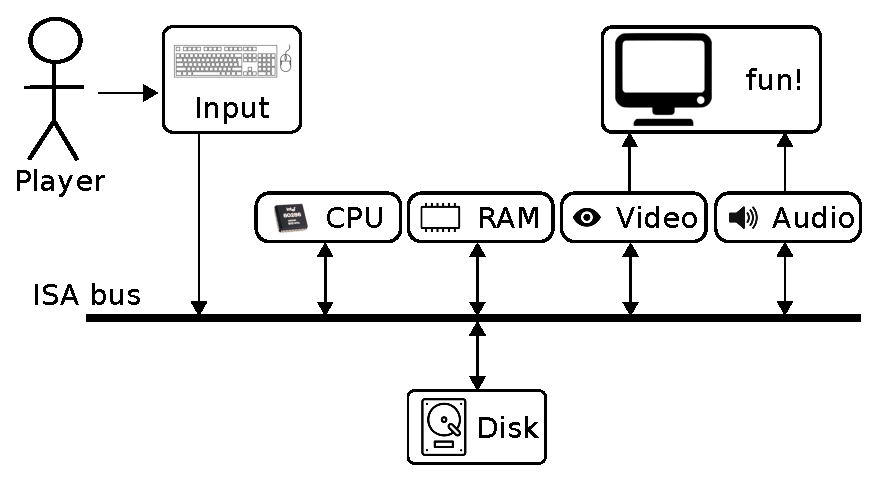
\includegraphics[width=1.0\textwidth]{imgs/drawings/fun_pipeline.eps}
\caption{IBM PC subsystems.}
\label{fig:digraph}
\end{figure}

\par
The IBM PC can be divided into six essential subsystems that determine the overall system performance and the gaming experience: 
\begin{itemize}
	\item CPU
	\item RAM
	\item Video
	\item Disk
	\item Audio
	\item Input devices
\end{itemize}
Each of these subsystems is described in this chapter.

\section{CPU: Central Processing Unit}
In the late 1980s, Intel’s x86 architecture dominated the IBM-compatible PC market, while Motorola’s 68000 series powered systems such as the Apple Macintosh, the Commodore Amiga, and workstations from Sun Microsystems. By 1989, approximately 15\% of US households owned a personal computer\footnote{https://www.statista.com/statistics/184685/percentage-of-households-with-computer-in-the-united-states-since-1984/}.


\subsection{Introduction of Intel x86 CPU}
  Intel released the 8086 in 1978, which was the first microchip of the successful x86 family line. One year later, in 1979, it released the 8088 which was a variant of the 8086. The main difference between the two is that there are only eight data lines for the external data bus in the 8088 instead of the 8086's 16 lines.  IBM chose the 8088 over the 8086 for its original PC/XT, because Intel offered a better price for the former and could supply more units. \\
  \par
  In 1982 Intel released the 80286 microchip, simply called the "286". A typical 8088 chip was running at 4.77MHz, where the 80286 was running at 6MHz and later popular versions at 12-16MHz. The 80286 was employed for the IBM PC/AT, introduced in 1984, and then widely used in most PC/AT compatible computers until the early 1990s\footnote{By the end of 1988, Intel estimates there were around 15 million 286-based PCs in use worldwide.}. It would be the last, fastest 16-bit PC processor Intel made. Its successor, the Intel 80386, was a true 32-bit processor with a 32-bit data bus.\\

 \par  
Although Commander Keen was 100\% compatible with the IBM-PC, it was hardly playable on an 8088 CPU. An 286 or higher was recommended to play the game primarily due to its reliance on the 16-bit data bus, as well as its raw speed. This section (and the bulk of this book) is written from the perspective of an 286 CPU, but most of the information is applicable to 8086, as well as PC's many generations newer.\\   

\begin{figure}[H]
\centering
  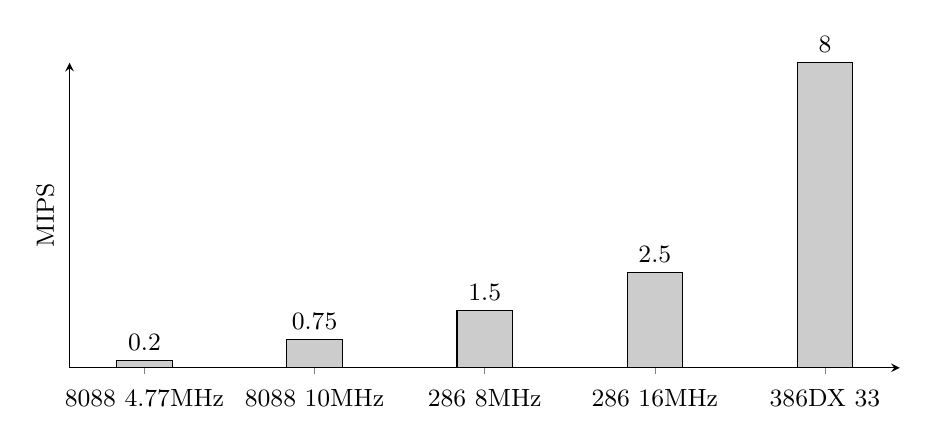
\begin{tikzpicture}[font=\small]
    \begin{axis}[
      width=1.0\textwidth,
      height=0.45\textwidth,
      ybar,
      bar width=20pt,
      ylabel={MIPS},
      ymin=0,
      ytick=\empty,
      xtick=data,
      axis x line=bottom,
      axis y line=left,
      enlarge x limits=0.11,
      symbolic x coords={8088 4.77MHz, 8088 10MHz, 286 8MHz,286 16MHz,386DX 33},
      xticklabel style={anchor=base,yshift=-\baselineskip},
      nodes near coords={\pgfmathprintnumber\pgfplotspointmeta}
    ]
      \addplot[fill=black!20,draw=black] coordinates {
		(8088 4.77MHz,0.2)      	
      	(8088 10MHz,0.75)
        (286 8MHz,1.5)
        (286 16MHz,2.5)
        (386DX 33,8)
      };
    \end{axis}
   
   \end{tikzpicture}
   \caption{Comparison\protect\footnotemark of CPUs with MIPS}
 \end{figure}
 \par
 % \addtocounter{footnote}{0}
  \footnotetext{Roy Longbottom's PC Benchmark Collection: http://www.roylongbottom.org.uk/mips.htm.}
   % \stepcounter{footnote}
 \par
  \trivia{A modern processor such as the Intel Core i7 3.33 GHz operates at close to 180,000 MIPS.}\\
  
  
\subsection{The Intel 80286}
  \begin{wrapfigure}[7]{r}{0.3\textwidth}
\centering
\vspace{-10pt}
\includegraphics[width=.3\textwidth]{imgs/drawings/intel_logo.eps}
\end{wrapfigure}
\par
The Intel 80286 chip is the CPU behind the original IBM PC AT (Advanced Technology). Other computer makers manufactured what came to be known as IBM clones, with many of these manufacturers calling their systems AT-compatible or AT-class computers. \\
\par
When IBM developed the AT, it selected the 286 as the basis for the new system because the chip provided compatibility with the 8088 used in the PC and the XT. Therefore, software written for those chips should run on the 286. The 286 chip is many times faster than the 8088 used in the XT, and at the time it offered a major performance boost to PCs used in businesses.\\

\par
The main reason the 286 computer was faster than its predecessor is that it executes instructions much more efficiently. An average instruction takes 12 clock cycles on the 8088, but takes an average of only 4.5 cycles on the 286 processor. Additionally, the 286 chip can handle up to 16 bits of data at a time through an external data bus twice the size of the 8088.\\

\par
\begin{figure}[H]
\centering
  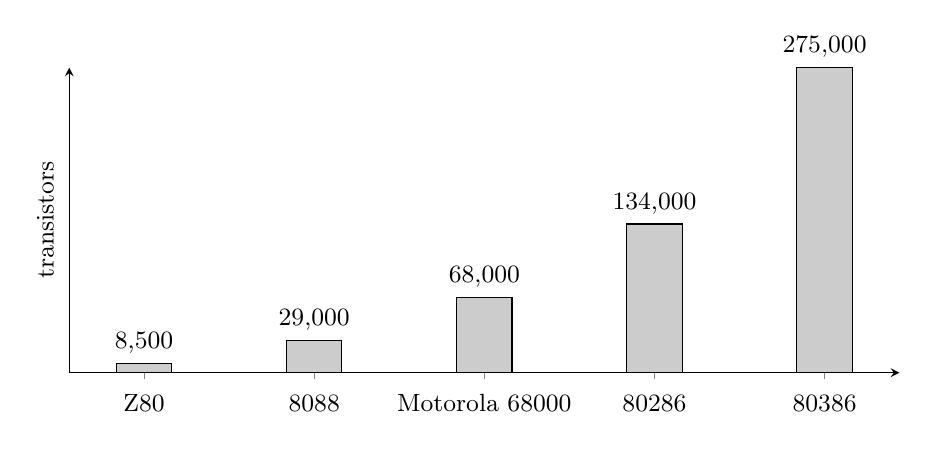
\begin{tikzpicture}[font=\small]
    \begin{axis}[
      width=1.0\textwidth,
      height=0.45\textwidth,
      ybar,
      bar width=20pt,
      ylabel={transistors},
      ymin=0,
      ytick=\empty,
      xtick=data,
      axis x line=bottom,
      axis y line=left,
      enlarge x limits=0.11,
      symbolic x coords={Z80, 8088, Motorola 68000,80286,80386},
      xticklabel style={anchor=base,yshift=-\baselineskip},
      nodes near coords={\pgfkeys{/pgf/number format/.cd,fixed}\pgfmathprintnumber\pgfplotspointmeta}
    ]
      \addplot[fill=black!20,draw=black] coordinates {
		(Z80,8500)      	
      	(8088,29000)
        (Motorola 68000,68000)
        (80286,134000)
        (80386,275000)
      };
    \end{axis}
   
   \end{tikzpicture}
   \caption{Comparison of CPUs with \# of transistors.}
 \end{figure}
 \par
  \trivia{Fast forward to today, the AMD Ryzen 9 7950X contains over 13 billion transistors.}\\


\par
The 286 CPU has two operating modes: real mode and protected mode. These modes are sufficiently distinct that the 286 can be regarded as two processors in one. In real mode, the 286 behaves essentially like an 8086 and is fully compatible with the 8088. In protected mode, however, the 286 introduced significant new capabilities. Programs designed to take advantage of this mode can access up to 16 MB of physical memory through its 24-bit address bus.\\

\par
A major limitation of the 286 is that it cannot switch from protected mode back to real mode without a hardware reset (a warm reboot) of the system. It can, however, switch from real mode to protected mode without a reset.\\

\trivia{Gordon Letwin of Microsoft found a way to switch back from protected to real mode, using a "triple fault"\footnote{https://en.wikipedia.org/wiki/Triple\_fault.} to soft reset the 286 CPU into real mode. However, it could take nearly 1 second, making switching from protected to real not feasible to be done often.}\\

\par
While the 8088 used a 3.0$\mu$m process, the 20286 used a 1.5$\mu$m process. The smaller process and increased surface (from 33mm$^2$ to 49mm$^2$) allowed Intel to pack 134,000 transistors on a 286 chip versus 29,000 on an 8088 chip.


\pagebreak
If you are holding a physical 9.25"x7.5" copy of this book, the CPU packaging is 25x25
mm square and the die is 7x7 mm, at 1:1 scale.\\


\fullimage{286_layout_photo.png}
\par 
\vspace{5pt}
% Below, a 1:1 scale of the 2.50cm x 2.50cm packaging next to a schematic showing the actual die inside.\\
\begin{minipage}{0.48\textwidth}
\centering
\scaledrawimage{2.50cm}{286_packaging.png} 
\end{minipage}
\hfill
\begin{minipage}{0.48\textwidth}
\centering
\scaledrawimage{2.50cm}{286_packaging_die.png}
\end{minipage}



 \pagebreak

\par 
To better understand why the 286 is much faster compared to the 8088, we need to understand the architecture of the chip. The 286 architecture can be summarized by four functional units as illustrated below.


\begin{figure}[H]
\centering
\includegraphics[width=\textwidth]{imgs/drawings/286_architecture.eps}
\caption{Internal block diagram of the 80286 processor}
\end{figure}
\par
The four functional units can be described by
\begin{itemize}
\item \textbf{Address Unit (AU)} is used to determine the physical addresses of instructions and operands which are stored in memory. The address lines derived by AU can be used to address different peripheral devices such as memory and I/O devices. 
\item \textbf{Bus Unit (BU)} interfaces the CPU with memory and I/O devices. The BU is used to fetch instruction bytes from the memory and stores them in the prefetch queue.
\item \textbf{Instruction Unit (UI)} receives instructions from the prefetch queue and an instruction decoder decodes them one by one. The decoded instructions are latched onto a decoded instruction queue.
\item \textbf{Execution Unit (EU)} is responsible for executing the instructions received from the decoded instruction queue. The EU consists of the register bank, arithmetic and logic unit (ALU) and control block. The ALU is the core of the EU and performs all the arithmetic and logical operations.\\
\end{itemize}

\par
The 8088 had a two-unit architecture consisting of the Execution Unit and the Bus Interface Unit. The introduction of four independent units operating in parallel was one of the primary reasons the 286 was significantly faster than the 8088.\\

\par
A good example is the calculation of physical memory addresses. In the 286, address calculations are performed by the dedicated address unit, whereas the 8088 computes effective addresses using the ALU, often consuming several additional clock cycles.\\

\par
\begin{figure}[H] 
\centering
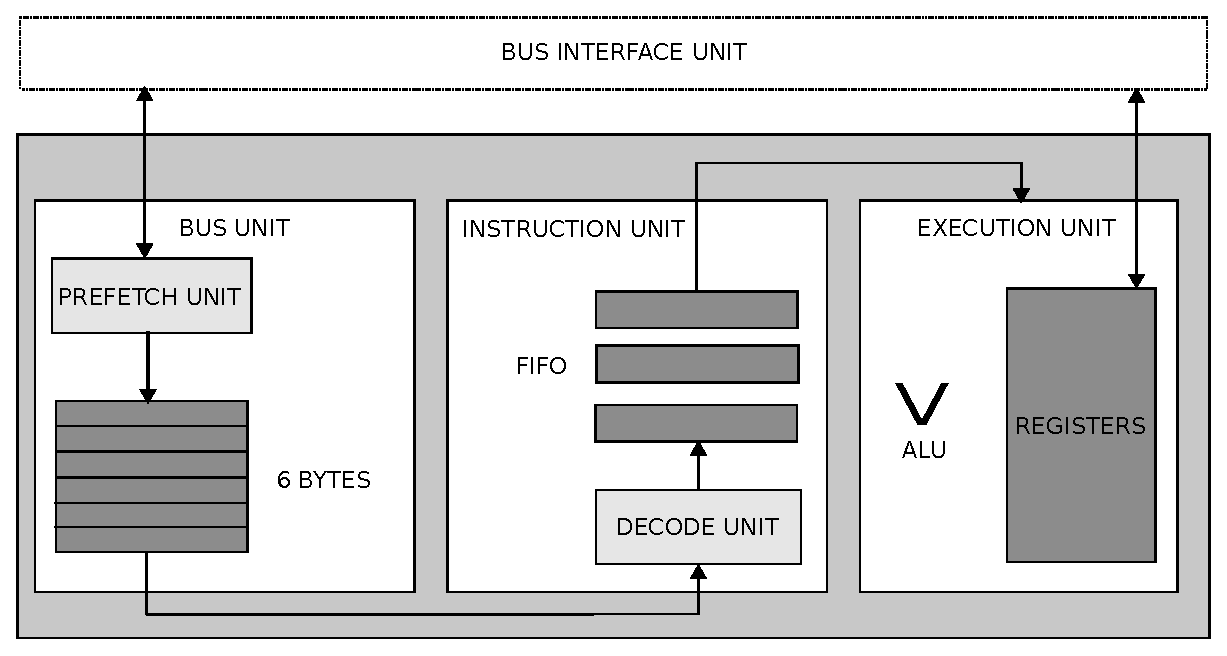
\includegraphics[width=\textwidth]{imgs/drawings/processing_unit.eps}
\end{figure}

\par
The remaining three units form a three stage pipeline. When the execution unit is not using the system bus, the bus unit fetches instructions and stores them in a 6-byte prefetch queue. The decode unit reads bytes from this queue, translates them into decoded instructions, and places them into a secondary three-instruction queue. Finally, the execution unit retrieves these decoded instructions and executes them.\\

\par
In practical terms, an 286 system running at the same clock frequency as an 8088 will typically be three to six times faster due to its pipelined architecture and dedicated functional units\footnote{https://www.tomshardware.com/reviews/processor-cpu-apu-specifications-upgrade,3566-6.html.}. \\

\par
The table below shows the average instruction costs for the 80286. Multiplication and division operations require significantly more cycles than most other instructions. For applications where every cycle counts, such as games, minimizing the use of multiplication and division during runtime was critical.\\

  \begin{figure}[H]
\centering  
\begin{tabularx}{\textwidth}{ X  Y }
  \toprule
  \textbf{Instruction type} &  \textbf{Clocks} \\
  \toprule 
   \cw{ADD reg8, reg8} & 2  \\
   \cw{INC reg8} & 2  \\
   \cw{IMUL reg16, reg16} & 24  \\
   \cw{IDIV reg16, reg16} & 28 \\
   \cw{MOV [reg16], reg16} & 5 \\
   \cw{OUT [reg16], reg16} & 3 \\
   \cw{IN [reg16], reg16} & 5 \\
  \toprule
\end{tabularx}
\caption{286 instruction costs\protect\footnotemark.}
\end{figure}
\addtocounter{footnote}{-1}
\stepcounter{footnote}
\footnotetext{Intel 80286 programmer's reference manual - 1987.}

\begin{figure}[H]
\centering
  \includegraphics[width=0.95\textwidth]{screenshots_300dpi/Intel80286.png}
\caption{The Intel 286, 7mm by 7mm packing 134,000 transistors}
\end{figure}

\par
For programming purposes, the 286 CPU can be summarized as follows::
\begin{itemize}
\item Arithmetic Logic Unit performing \cw{add}, \cw{sub}, \cw{mul}, etc.
\item 14 registers, all 16-bits wide:
\begin{itemize}
  \item General Purpose Registers: AX, BX, CX, DX
  \item Index Registers: SI, DI, BP, SP
  \item Segment Registers: CS, DS, ES, SS
  \item Status and Control Register
  \item Program Counter: IP
\end{itemize}
\item A 24-bit address bus for up to 16MiB of addressable RAM
\item Memory Management Unit (MMU), used in Protected Mode
\end{itemize}
 \par



\section{RAM}
When the first IBM PC was introduced in 1981, it came with a base memory of 16 KiB or 64 KiB and could be expanded up to 256 KiB\footnote{This book uses IEC notation where KiB is $2^{10}$ and KB is $10^3$.}. This was a large amount of memory at the time, considering that the average home computer, such as the Commodore 64 or MSX systems, contained a maximum of 64 KiB. With the introduction of the 8088 CPU and the IBM XT, the maximum memory increased to 640 KiB. Later, with the introduction of the 80286, one could, in theory, address up to 16 MiB of memory. In practice, however, this was never fully utilized due to the constraints of the DOS operating system.\\


\subsection{x86 Real and Protected Mode}
With the 16-bit architecture of the 8088, only 64 KiB could be addressed using a single 16-bit address register. To address more memory, Intel introduced the "Real Mode" architecture. It combined two 16-bit address values into a 20-bit physical address, thereby providing access to up to 1 MiB of RAM. There was no memory protection and direct access to all hardware, meaning that applications could (un)intentionally overwrite each other’s memory.\\

\par
As memory requirements increased, there was a need for an improved CPU architecture supporting larger address spaces and access protection. With the introduction of the 80286, Protected Mode was added to the architecture. It provided 24-bit memory addressing, allowing up to 16 MiB of memory, along with memory protection through an MMU that prevented applications from accessing or overwriting memory belonging to other programs.\\

\par 
To maintain backward compatibility with older software, the 80286 also retained Real Mode. The system always booted in Real Mode and could then switch to Protected Mode. A significant failing of the 80286 chip is that it cannot switch back from protected mode to real mode without a hardware reset (a warm reboot) of the system.\\


\trivia{Gordon Letwin of Microsoft found a way to switch back from protected to real mode, using a "triple fault"\footnote{https://en.wikipedia.org/wiki/Triple\_fault.} to soft reset the 286 CPU into real mode. It could take nearly 1 second, making switching from protected to real not feasible to be done often.}\\

\par
The protected mode could not run existing MS-DOS software. To use it, a completely new operating system had to be rewritten, and there was little incentive for developers to do this when they could target the 8086, which held the largest market share. As a result, developers on DOS continued programming within the limitations of the 8088 architecture, where only 1 MiB of RAM could be addressed without memory protection.\\

\par
To make matters worse, only the first 640 KiB of the 1 MiB address space was available for applications. This area, also called Conventional Memory, included system-specific data, the DOS operating system, as well as drivers needed to run the system (e.g., a mouse driver), which effectively left \textasciitilde{}620 KiB of usable memory for applications. The remaining 384 KiB, known as the Upper Memory Area (UMA), was reserved for video memory, BIOS ROM, and memory-mapped I/O.\\


\par
\begin{figure}[H]
\centering
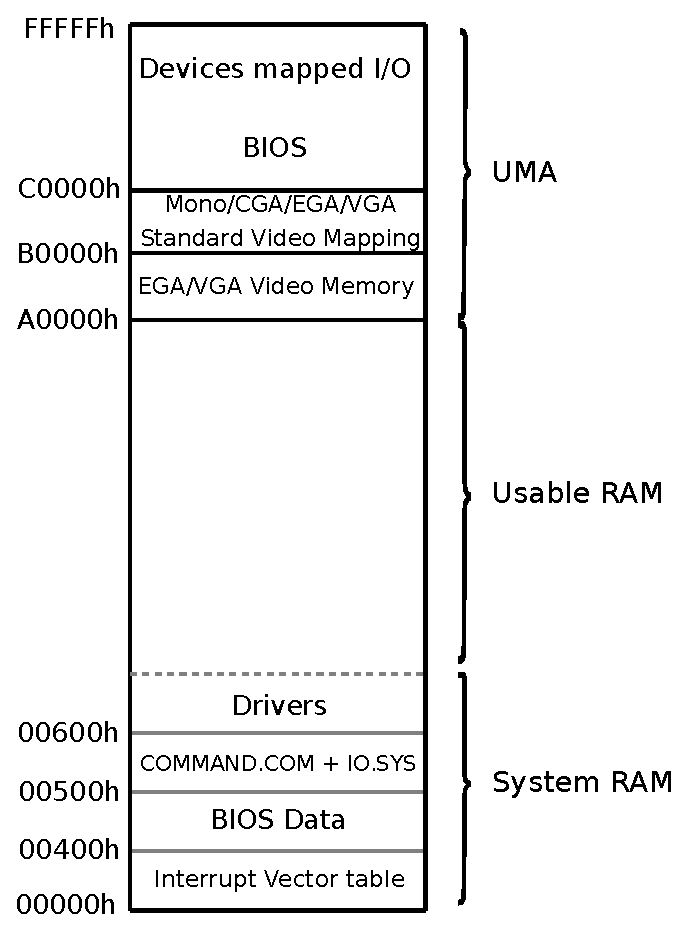
\includegraphics[width=0.8\textwidth]{imgs/drawings/real_mode_v2.eps}
\caption{First 1MiB of RAM layout.} 
\label{fig:fp_internals}
\end{figure}



\subsection{Memory addressing}
If Intel had allowed the CPU to combine two registers into a high and low pair of 32-bits, it could have referenced up to 4 GiB of memory in a linear fashion. Keep in mind, however, this was at a time when many never dreamed we'd need a PC with more than 640 KiB of memory for user applications and data.\\

\par
\begin{fancyquotes}
I've said some stupid things and some wrong things, but not "640K is enough". No one involved in computers would ever say that a certain amount of memory is enough for all time.\\ 
\par
\textbf{Bill Gates - Founder of Microsoft}
\end{fancyquotes}\\


\par
So, instead of dealing with whatever problems a linear addressing scheme of 32-bits would have produced, they created the segment:offset scheme 
which allows a CPU to effectively address 1 MiB\footnote{This book uses IEC notation where MiB is $2^{20}$ and MB is $10^6$.} of memory. The segment:offset schema combines two 16-bit registers, one designating a segment and the other an offset within that segment.
\\

\par
\begin{figure}[H]
\centering
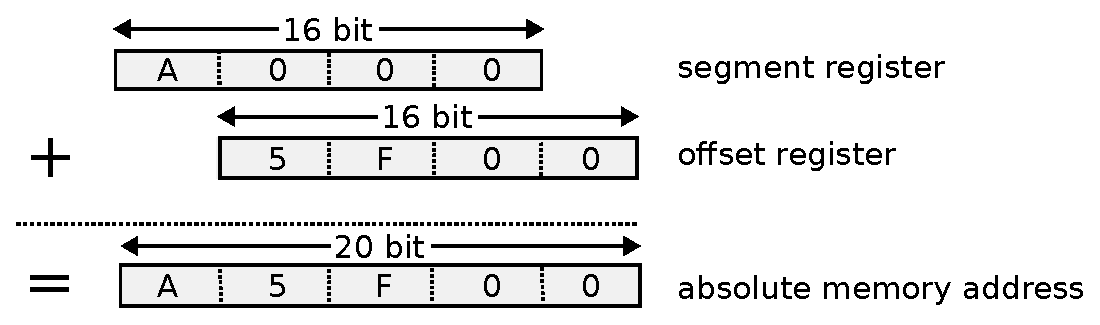
\includegraphics[width=\textwidth]{imgs/drawings/register_combination_20_bits_address.eps}
\caption{How registers are combined to address memory.}
\label{fig:register_comb_to_20_bits}
\end{figure}
\par

To support this architecture, four segment registers are introduced. Each of these segment registers has its own purpose:
\begin{itemize}
  \item CS segment register, where the machine code (instructions) reside.
  \item DS segment register, where the data resides.
  \item SS segment register, where the stack resides.
  \item ES segment register, which is used as extra data segment.
\end{itemize}

\par
In C-language a memory address can be accessed directly using pointers. A pointer is a variable that stores the memory address of another variable as its value. There are two kinds of pointers: "near" and "far". \\

\par
A near pointer refers to a function or data object that is within the default code or data segment. It is 16 bits long and contains an offset into the current DS data segment if it's a data pointer, or into the current CS code segment if it's a function pointer. A far pointer could refer to a function or data that is in a different segment than the current, default segment. It is 32 bits long and contains a segment and offset, which identifies the location where the code or data is stored. \\

\par
\begin{figure}[H] 
\centering
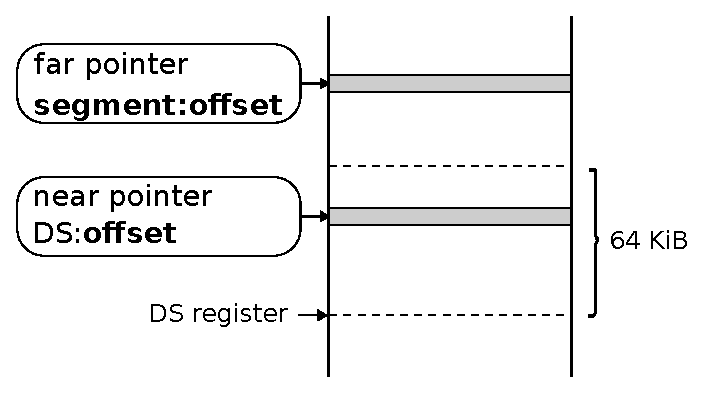
\includegraphics[width=0.7\textwidth]{imgs/drawings/near_far_pointer.eps}
\end{figure}

\par
Accessing code or data with a near pointer is much faster than using a far pointer. When you use a near pointer, the program only needs to locate the code or data through the offset (or index) register. However, when using a far pointer, the program must first find the segment and then locate the code or data within that segment. For faster execution, one should use as many near pointers as possible. The drawback of using only near pointers is that they limit the program or data to 64KiB of memory.\\

\par
It's important to note that a far pointer increments only the offset, not the segment. If you iterate over a data array larger than 64KiB, there will be no automatic overflow handling, meaning you can only address up to 64KiB of memory. \\

\par
\begin{minipage}{\textwidth}
 \lstinputlisting[language=C]{code/far_pointer.c}\par
 \end{minipage}\\
\par
Will output:\\
\par
\begin{minipage}{\textwidth}
 \lstinputlisting[language=C]{code/far_pointer_out.c}\par
 \end{minipage}

\par
To work with memory beyond this limit, you can use another type of pointer called a "huge" pointer, which allows pointer arithmetic to function correctly beyond the 64KiB boundary.\\

\par
\begin{minipage}{\textwidth}
 \lstinputlisting[language=C]{code/huge_pointer.c}\par
 \end{minipage}\\
\par
Will output the address:\\
\par
\begin{minipage}{\textwidth}
 \lstinputlisting[language=C]{code/huge_pointer_out.c}\par
 \end{minipage}\\
\par

The huge pointer is based on the absolute (or linear) 20-bit memory location and \\ \mbox{segment:offset} normalized address. The absolute memory address can be calculated by\\

\par
\begin{minipage}{\textwidth}
\lstinputlisting[ language={[x86masm]Assembler}]{code/segment_offset}
\end{minipage}\\

\par
For example, the absolute address of \cw{A000:002F} is \cw{A0000h} + \cw{002Fh} = \cw{A002Fh}. By confining the offset to just the hexadecimal values \cw{0h} through \cw{Fh}, we have a unique way to reference all segment:offset memory pair locations. This results in the normalized address \cw{A002:000F}. A huge pointer is normalized when pointer arithmetic is performed on it. \\
\par
\begin{minipage}{\textwidth}
 \lstinputlisting[language=C]{code/huge_pointer_normalized.c}\par
 \end{minipage}\\
\par
Will output:\\
\par
\begin{minipage}{\textwidth}
 \lstinputlisting[language=C]{code/huge_pointer_norm_out.c}\par
 \end{minipage}\\
\par


\trivia{Since the normalized form will always have three leading zero bytes in its offset, programmers often write it with just the digit that counts: \cw{AFFF:F}}\\

\par
A \cw{huge} reference is much slower than the \cw{far} reference as it comes with additional overhead to update the segment and address normalization after every arithmetic manipulation. So, most programmers avoided the \cw{huge} pointer, unless really needed.\\




\subsection{Real mode: Memory models}
When a program is compiled and executed, the operating system allocates a chunk of memory to the program. This memory is divided into different segments, aligned with the segment registers:
\begin{itemize}
  \item \textbf{Code section}: Stores the program executable. When you compile a C program, the compiler converts your code into assembly instructions that the CPU executes.
  \item \textbf{Data section}: Stores initialized and uninitialized global and static variables.
  \item \textbf{Stack section}: Memory used for local variables and data inside functions. The stack grows downwards, towards lower memory addresses.
  \item \textbf{Heap section}: Memory that is dynamically allocated using the \cw{malloc()} function. The heap typically grows upwards, meaning it expands towards larger memory addresses.
\end{itemize}

\par
The x86 real mode provides different memory segment layouts, called "memory models". Each memory model determines how segments are organized and defines whether the default pointer type for functions and data is near or far. A near pointer automatically associates with one of the segment registers. Six memory models\footnote{See Borland C++ 3.1 Programmer's guide, section DOS Memory management.} exist, each offering trade-offs between minimum system requirements, maximizing code efficiency, and accessing available memory.


\begin{figure}[H]
\renewcommand{\arraystretch}{1.7}
\centering
\begin{tabularx}{\textwidth}{ X X X X X >{\hsize=.3\textwidth}Y} 
  &  \multicolumn{2}{c}{\textbf{Default pointer type}} & \multicolumn{2}{c}{\textbf{Size}} &  \\ \cline{2-5}
 \textbf{Model}   & \textbf{Code} & \textbf{Data} & \textbf{Code} & \textbf{Data} & \textbf{Definition} \\ \hline
 Tiny & near & near & \multicolumn{2}{c}{<64KiB} & CS=DS=SS \\ \hline
 Small & near & near & <64KiB & <64KiB & DS=SS \\ \hline
 Medium & far & near & >64KiB & <64KiB & DS=SS, multiple code segments \\ \hline
 Compact & near & far & <64KiB & >64KiB & single code segment, multiple data segments\\ \hline
 Large & far & far & >64KiB & >64KiB & multiple code and data segments \\ \hline
 Huge & far & far & >64KiB & >64KiB & multiple code and (global) data segments \\ \hline 

\end{tabularx}\\
\end{figure}

\pagebreak
The smallest is the "tiny memory model", where all three segment registers (CS, DS, SS) start at the same memory location. The first part of memory is used for code instructions, followed by the data section. The heap begins directly after the data section, and the stack starts at the opposite end of the segment, growing downward. Both the heap and stack can dynamically grow or shrink during program execution. If they continue to grow, they may eventually collide, causing a system or application crash. \\

\begin{figure}[H]
\centering
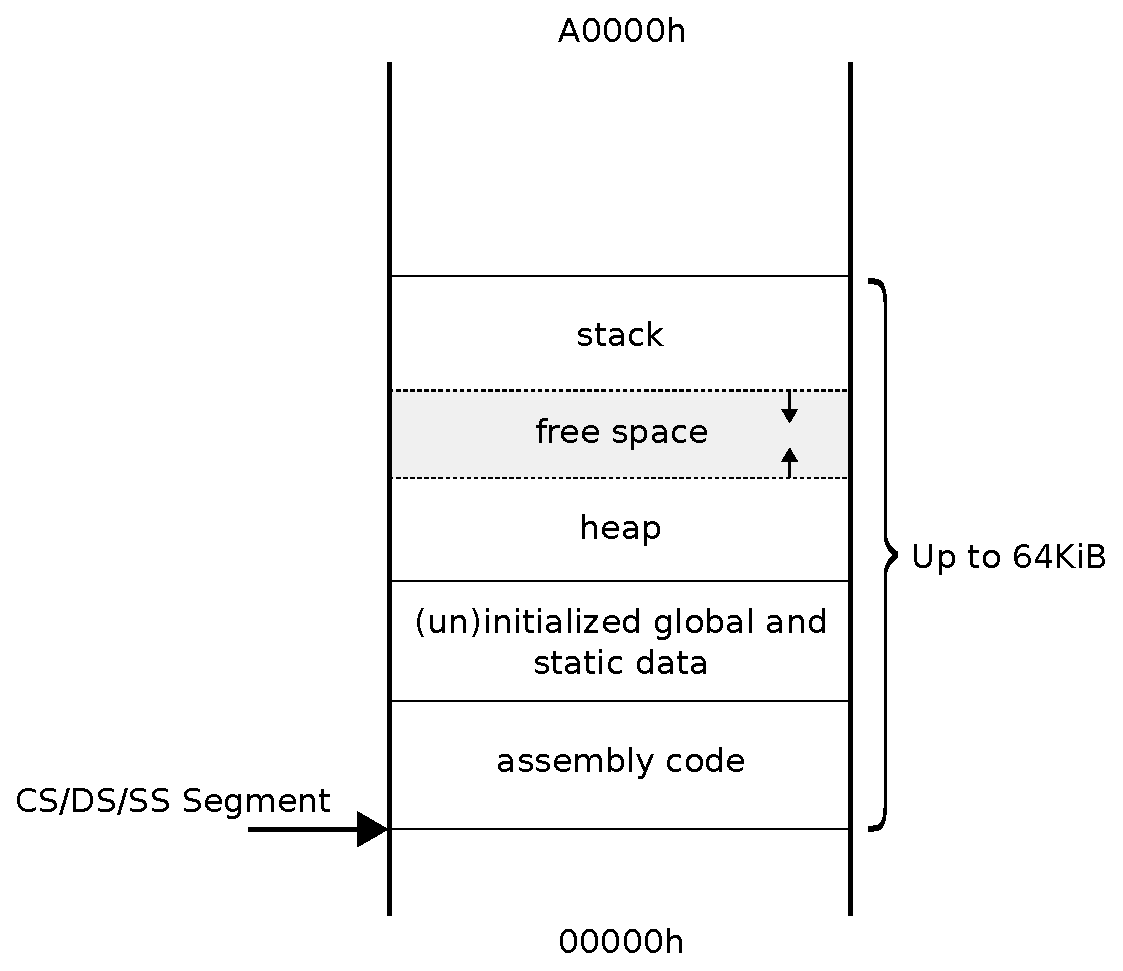
\includegraphics[width=0.75\textwidth]{imgs/drawings/memory/tiny_mm.eps}
\caption{Tiny memory model layout.}
\label{fig:mm_tiny}
\end{figure}

\par
All functions and data are accessed using near pointers, meaning the segment registers are set once and never changed during execution. However, this limits the program to a maximum of 64KiB, like programming on a 16-bit system.\\

\trivia{The tiny memory model was required by programs that ended with the .COM extension, and it existed for backward compatibility with CP/M operating system. CP/M ran on the 8080 processor which supported a maximum of 64KB of memory.}\\

\par
In the "small memory model", instructions and data are separated, each having its own 64KiB segment. The code segment can store up to 64KiB of instructions, while the global data, stack, and heap share a separate 64KiB segment. Code execution is efficient since both functions and data are accessed using offset registers (near pointers) only.\\


\begin{figure}[H]
\centering
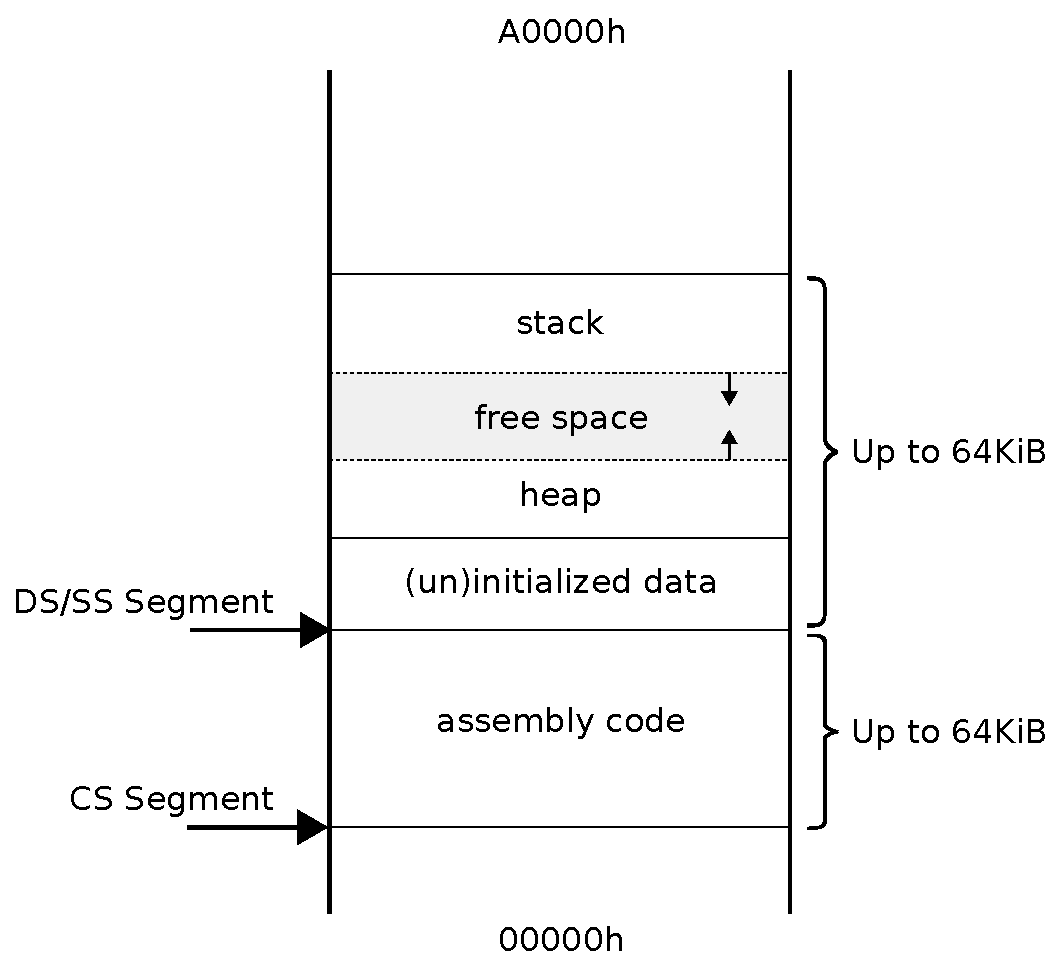
\includegraphics[width=0.7\textwidth]{imgs/drawings/memory/small_mm.eps}
\caption{Small memory model layout, code and data each have 64KiB.}
\label{fig:mm_small} 
\end{figure}

\par
The "medium memory model" is ideal for programs with a large amount of code but minimal data. Many computer games fell into this category, since they had a lot of game logic, but not a lot of (global) game state data. In this model, each C source file has its own code segment, allowing up to 64KiB per file. A table manages all code segment references, with the CS register pointing to one segment at a time. Each function is a far pointer by default, requiring both the CS segment and IP offset register to be updated. While this model supports larger codebases, it comes at the cost of slower execution due to the far pointers.\\

\trivia{When compiling a source file, its code cannot exceed 64KiB, as it must fit inside one code segment. If the file is too large, the program must be broken into smaller source files and compiled separately.}\\

\par
The "compact memory model" is the opposite of the medium memory model, allowing more than 64KiB of data while restricting function code to 64KiB. The "large memory model" supports both code and data larger than 64KiB but requires far pointers for both, leading to slower execution. The "huge memory model" removes the 64KiB limit on global data, allowing more flexibility, but also incurs a performance penalty. A detailed layout and explanation of each memory model is described in Appendix \ref{appendix_memory_models}.\\

\begin{figure}[H]
\centering
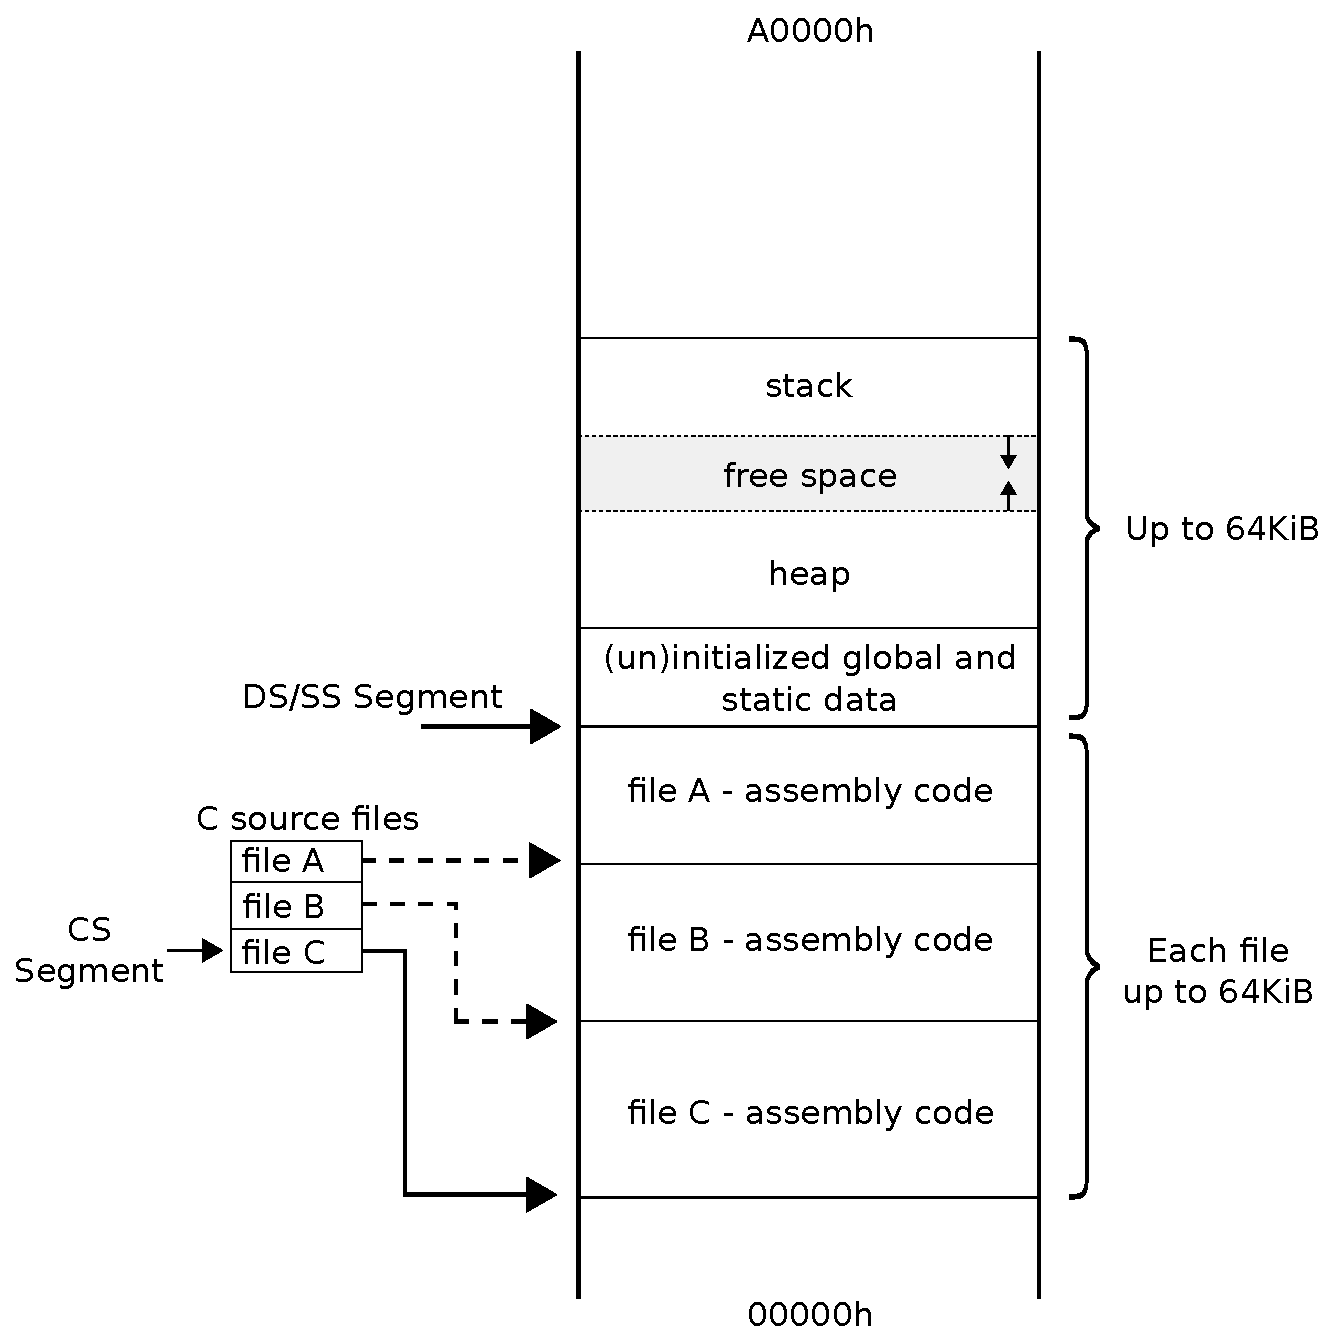
\includegraphics[width=0.85\textwidth]{imgs/drawings/memory/medium_mm.eps}
\caption{Medium memory model layout, code can be larger than 64KiB.}
\label{fig:mm_medium}
\end{figure}

\bigskip


\subsection{Mixed Model Programming}

In the medium memory model, the data segment remains limited to 64KiB. For most games, this is enough to store game state variables. However, the size of the heap is far too small to store game data such as graphics and game maps. One option is to use the large or huge memory models, but these come with the downside of slower data access due to the use of far pointers for all data.\\


\par
Fortunately, there is a way to access additional memory using the medium model. A large portion of unallocated memory is available between the stack and the high address \cw{A0000h}. This memory, known as the "far heap", can be allocated using the \cw{farmalloc()} function. This technique, called mixed model programming, combines the advantages of one of the six standard memory models with custom near and far pointer allocation. In the case of the medium memory model, it allows the program to benefit from near pointer efficiency for global data and the stack, while also providing sufficient memory for dynamically allocated assets like graphics and game maps.\\


\begin{figure}[H]
\centering
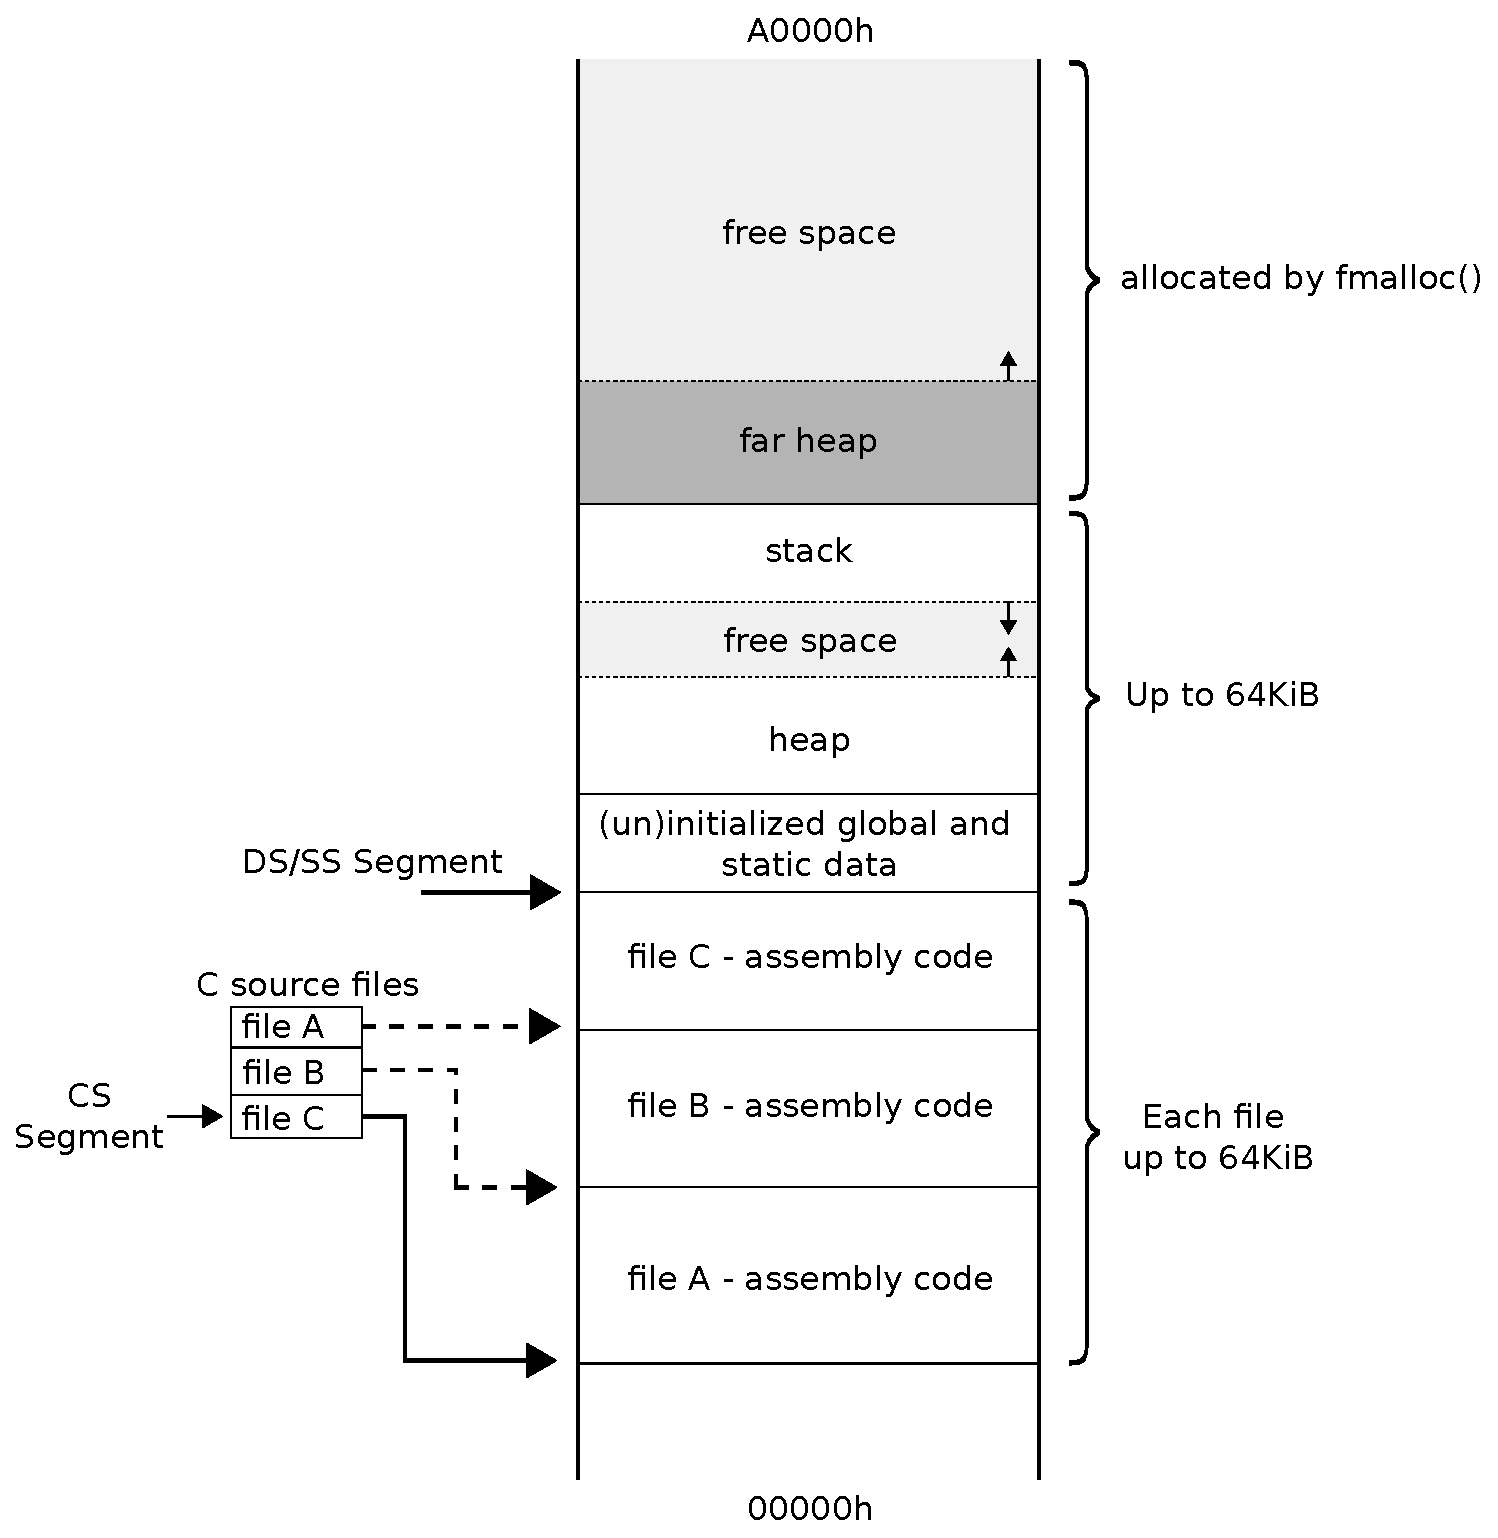
\includegraphics[width=1.0\textwidth]{imgs/drawings/memory/farheap_medium_model.eps}
\caption{Medium memory model layout with far heap memory.}
\label{fig:mm_farheap}
\end{figure}
 

\subsection{16-bit Data alignment}
Compared to the Intel 8088, the 286 CPU contained a 16-bit external data bus where the 8088 only had an 8-bit bus. Thanks to its 16-bit bus, the 286 can access and write word-sized memory variables just as fast as byte-sized variables. There's a catch, however: this is only true for word-sized variables that start at even memory addresses. When the 286 is asked to perform a word-sized access starting at an odd memory address, it actually performs two separate accesses, each of which fetches 1 byte, just as the 8088 does for all word-sized accesses. In other words, the effective capacity of the 286's external data bus is halved when a word-sized access to an odd address is performed\footnote{See Michael Abrash's Graphics Programming Black Book Special Edition, chapter 11.}.\\

\begin{figure}[H]
\centering
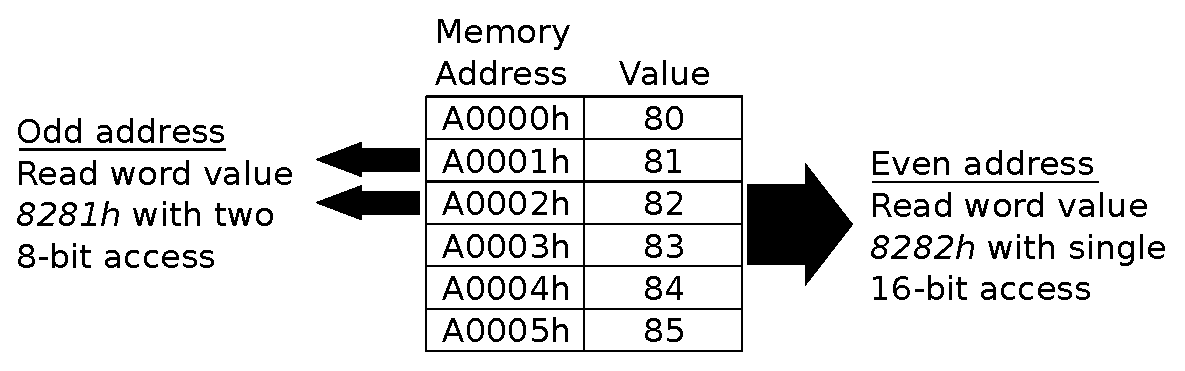
\includegraphics[width=0.85\textwidth]{imgs/drawings/data_alignment.eps}\\
\end{figure}
\par
 
\par
The way to deal with the data alignment cycle-eater is straightforward: Don't perform word-sized access to odd addresses on the 286 if you can help it. This is not an issue for small memory operations, but it will harm performance when copying large memory blocks. 


\section{Video}

Unlike home computers, the IBM PC did not include onboard video hardware. Instead, it required a separate video adapter card, which was installed in one of the system’s expansion slots. Each video adapter was typically paired with its own dedicated CRT monitor—a large, heavy display, usually with a 14" diagonal screen.\\


\subsection{Inner workings of a CRT monitor}

The first computer monitors were built around a Cathode Ray Tube (CRT). The picture on a CRT is generated by an electron gun, which converts electrical power into a narrow beam of electrons moving with substantial kinetic energy. The inside of the screen is coated with phosphor, which glows when struck by the electron beam (and for a short time thereafter).\\

\par
The electron beam is highly susceptible to magnetic fields, allowing it to be deflected using magnets. By placing horizontal and vertical electromagnets around the neck of the tube (the deflection yoke), the beam can be positioned anywhere on the screen. Manually controlling the beam would be tedious and impractical, so this process is automated by connecting the electromagnets to an oscillator that generates sawtooth waveforms.\\

\begin{figure}[H]
\centering
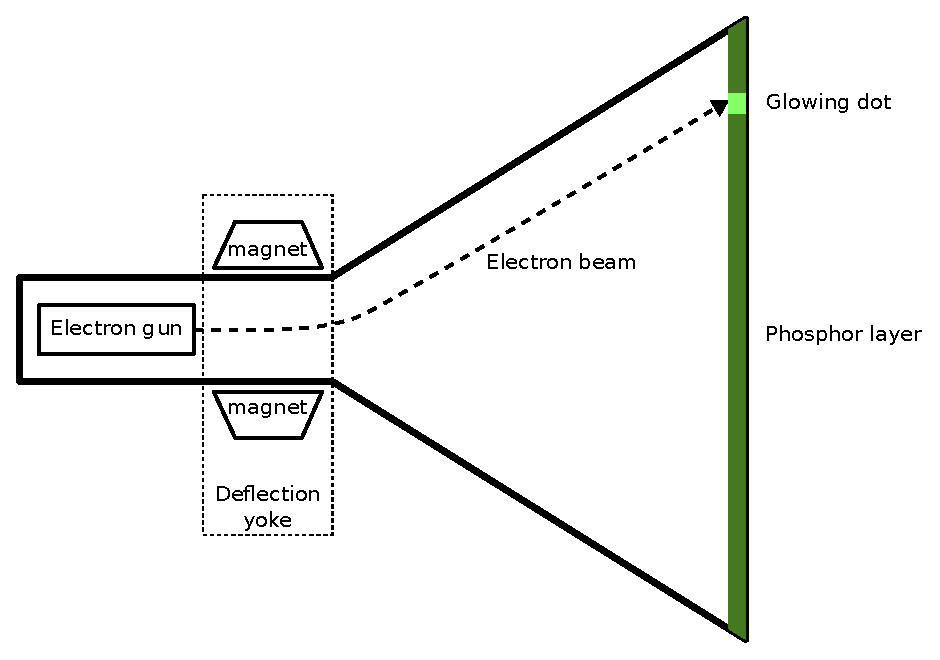
\includegraphics[width=1.0\textwidth]{imgs/drawings/CRT_inner.eps}
\caption{Inner working of CRT monitor.}
\label{fig:CRT_inner_working}
\end{figure}



\par
When both oscillators run together at precisely controlled frequencies, the electron beam scans the phosphor-coated screen from left to right and from top to bottom. The vertical oscillator determines how often the entire screen is redrawn, also known as the refresh rate. If the refresh rate is too low, the display will flicker. Most people can perceive flicker when the refresh rate drops below about 60 Hz, which is why most CRT displays operate at a  refresh rate of 60 Hz or higher.\\

\par
The CGA standard has a maximum vertical resolution of 200 lines, which requires the horizontal oscillator to operate at a much higher frequency of approximately 12 kHz in order to maintain a 60 Hz refresh rate. Standard CGA monitors are equipped with a horizontal frequency of 15.75 kHz, which is sufficient to refresh 200 lines. EGA monitors support two synchronization modes: the CGA-compatible 15.75 kHz / 60 Hz mode, and an EGA-specific horizontal rate of 21.85 kHz to support the newer 350-line display.\\

\trivia{The 15.75 kHz horizontal frequency is the standard used for NTSC television signals in North America and Japan. By adopting this frequency rate, IBM made it possible to connect a CGA card to standard televisions.}\\

\par
To generate an image, the output of the electron gun is modulated on and off, controlling which regions of phosphor get hit and which don’t. Each horizontal sweep of the beam is called a scan line. The time during which the beam returns to the left edge of the screen is known as the horizontal retrace, while the time required to return to the top is called the vertical retrace.\\

\begin{figure}[H]
\centering
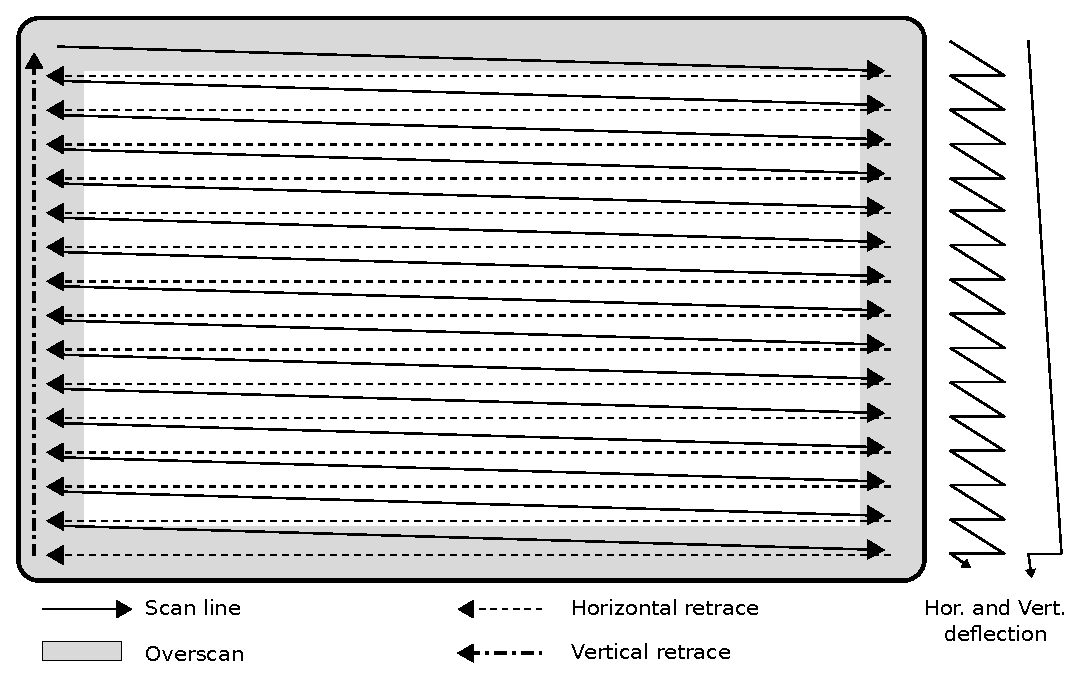
\includegraphics[width=1.0\textwidth]{imgs/drawings/monitor.eps}
\caption{Horizontal/vertical oscillator and CRT monitor scan.}
\label{fig:CRT_monitor_scan}
\end{figure}


\par
The electron beam cannot instantly stop and reverse direction; it must slow down, change direction, and accelerate again at the edges of the screen. This is handled by moving the beam outside the visible display area during retrace. This practice, known as overscan, intentionally directs the beam over regions of the screen that are not visible to the viewer, resulting in an image that is slightly larger than the active display area (the area which contains the actual character and/or graphics data).

\subsection{And then there was color} 
So far, this explanation has described a monochrome display, which uses a single color of phosphor. To produce a color image, the screen is coated with a red, a green, and a blue phosphor, arranged in a triangular shape. \\

\par
The color CRT contains three separate electron guns, each responsible for one of the RGB components of the image. In the figure below, the rays from the cannons are colored so the reader can follow, but electrons have no color. To ensure that each electron beam strikes only the phosphor of its corresponding color, a shadow mask is placed between the electron guns and the phosphor-coated screen.\\

\begin{figure}[H]
\centering
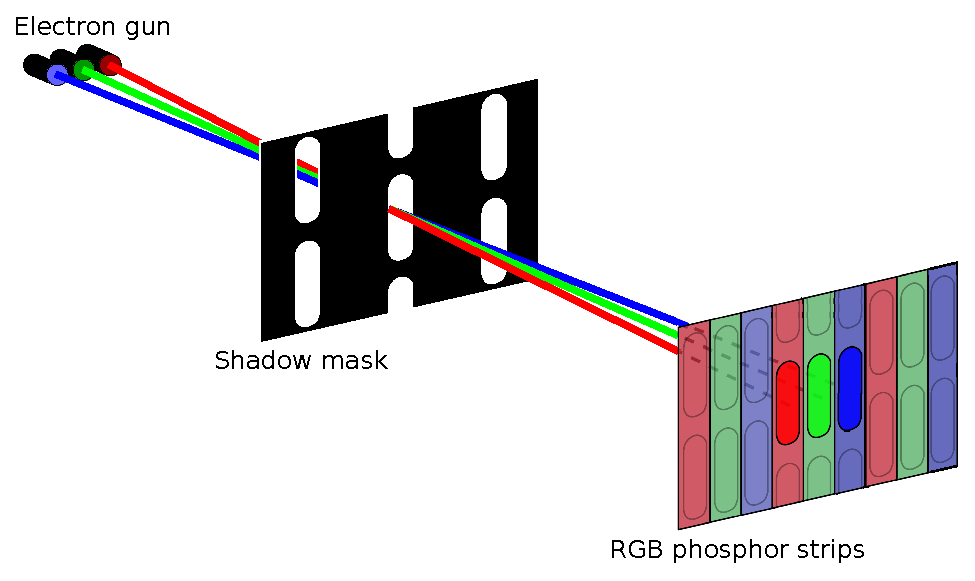
\includegraphics[width=1.0\textwidth]{imgs/drawings/CRT_color_display.eps}
\caption{CRT color display. }
\label{fig:CRT_color}
\end{figure}

\par
The distance between the same-colored phosphor dots on the screen is called the "dot pitch". It dictates the image sharpness and for the EGA monitor it generally ranged from 0.28mm to 0.40mm.\\

\par
The three dots in a triangle gives the appearance of discrete pixels, but in practice it is nearly impossible to control individual phosphor elements directly. Take the example of Figure \ref{fig:CRT_dot} where we light up green. The beam, represented by the circle, will usually hit multiple adjacent green phosphor elements at once. As a result, the effective “dot” (or pixel)—the smallest addressable unit of information on the screen—is defined by the combined effects of the RGB phosphor pattern density and the diameter of the electron beam.\\

\begin{figure}[H]
\centering
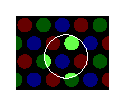
\includegraphics[width=0.43\textwidth]{imgs/drawings/CRT_dot.eps}
\caption{"dot" or "pixel" on a CRT screen. }
\label{fig:CRT_dot}
\end{figure}

\par
Everything described up to this point occurs entirely inside the monitor. This is where the video adapter comes into play, controlling the display via the DE-9 video connector.\\

 \begin{figure}[H]
\centering
\includegraphics[width=0.15\textwidth]{imgs/drawings/ports/DE9_serial_port.eps}
\caption{DE-9 video output connector.}
\label{fig:serialPort}
\end{figure}

\par
The CGA and EGA adapters use
\begin{itemize}
	\item Two pins for horizontal and vertical synchronization signals 
	\item Four (CGA) or six (EGA) pins to control the intensity of the electron guns
\end{itemize}
The horizontal and vertical synchronization pins carry timing signals that match the monitor’s operating frequencies (15.7 kHz / 60 Hz for CGA, and 21.85 kHz / 60 Hz for EGA's high-resolution mode). The monitor listens for these signals, synchronizes its internal oscillators to them, and deflects the electron beam accordingly.\\

\par
The CRT draws each scan line from left to right, while the control pins from the video adapter determine which portions of the scan line are illuminated. When a scan line is completed, the video adapter generates a horizontal synchronization pulse (HSYNC), to indicate a return to the left side of the screen. This process continues line by line until the bottom of the screen is reached. At that point, the adapter generates a vertical synchronization pulse (VSYNC), and the electron beam retraces back to the top of the screen to begin drawing the next frame.\\

\pagebreak
\subsection{History of Video Adapters}

The original IBM PC and XT could choose between the Monochrome Display Adapter (MDA) and the Color Graphics Adapter (CGA) expansion cards. With the introduction of the IBM PC AT in 1984, IBM introduced the Enhanced Graphics Adapter (EGA). Three years later, the EGA was succeeded by the Video Graphics Array (VGA).\\


\bigskip
 \begin{figure}[H]
\centering  
\begin{tabularx}{\textwidth}{ l X l Y }
  \toprule
  \textbf{Name} &  \textbf{Year Released} & \textbf{Memory} & \textbf{Max Resolution}\\
  \toprule \codeword{MDA}
   (\textbf{M}onochrome
   \textbf{D}isplay
   \textbf{A}dapter) & 1981 & 4KiB & 80x25\footnotemark 
   \\ \codeword{CGA}
   (\textbf{C}olor
   \textbf{G}raphics
   \textbf{A}dapter) & 1981 & 16KiB & 640x200
   \\ \codeword{Hercules} & 1982 & 64KiB & 720x348
    \\ \codeword{EGA}
   (\textbf{E}nhanced
   \textbf{G}raphics
   \textbf{A}dapter) & 1984 & 64KiB & 640x350
   \\ \codeword{VGA}
   (\textbf{V}ideo
   \textbf{G}raphics
   \textbf{A}rray)  & 1987 & 256KiB & 640x480
    \\
  \toprule
\end{tabularx}
\caption{Video interface history.}\label{fig:vga_history}
   
\end{figure}
\addtocounter{footnote}{-1}
\stepcounter{footnote}
\footnotetext{Text mode only.}

The EGA represented an interesting middle ground for game developers in the late 1980s and early 1990s. It supported a sufficiently high display resolution and enough colors to produce respectable games. However, programming the EGA proved to be incredibly difficult. The card has many dark corners and undocumented behaviors.  To fully master the hardware, one must delve deeply into its inner workings.\\


\subsection{Introduction of EGA Video Card}

IBM introduced the Enhanced Graphics Adapter (EGA) in 1984 as the successor of CGA. The standard card was shipped with only 64KiB video memory, but it had the option to expand the memory using the onboard graphics memory expansion card.
Figure \ref{fig:ibm_ega_card} shows the original IBM EGA card, a clunky beast full of discrete components. The memory consists out of TMS4416 RAM, a common memory chip for (home) computers around that period. Each chip contains 16KiB of 4-bits memory, so one needs two chips to end up having 16KiB of 8-bit memory and eight chips for 64KiB of 8-bit memory. \\

\trivia{Texas Instruments introduced the first 16KiB by 4-bits as TMS4416 in 1980\footnote{https://pdf1.alldatasheet.com/datasheet-pdf/view/103706/TI/TMS4416.html}. Still, it took until 1984 until they became widely available and lower priced than four TMS4116 chips (16KiB by 1-bit). However, at that time 64 KiB RAM was the way to go for new designs. Computers with only 16 KiB as base memory - and that's where TMS4416 would have been a cost saver - were already on the way out.}\\

\begin{figure}[H]
  \centering 
  \includegraphics[width=1.3\textwidth, angle =90 ]{screenshots_300dpi/hardware/ibm_ega_card.png} 
  \caption{Original IBM EGA card}
  \label{fig:ibm_ega_card}
\end{figure}




\par
To add additional video memory to the IBM EGA card a Graphics Memory Expansion Card could be purchased. By default, only the bottom row of memory was populated with chips, expanding the total EGA video memory to 128KiB. The expansion card provided dual in-line package (DIP) sockets for further memory expansion. Populating the DIP sockets with a Graphics Memory Module Kit adds two additional rows of 64KiB, bringing the EGA memory to its maximum of 256KiB. \\


\begin{figure}[H]
  \centering 
  \includegraphics[width=1.0\textwidth]{screenshots_300dpi/hardware/ibm_ega_graphics_memory_expansion_card.png} 
  \caption{EGA Memory Expansion Card, bottom row populated with memory chips.}
  \label{fig:ibm_ega_card}
\end{figure}

\vspace{5pt}
\par
The EGA clones that started coming along in 1986-87 were based on integrated chipsets, and the vast majority of them came with the maximum of 256KiB on board. When Commander Keen came out, the headcount of EGA cards with less than 256KiB would've been practically negligible\footnote{PC Tech Journal Oct 1986 (page 82-83) and PC Tech Journal Nov 1986 (page 148-149)}.\\

\par
The next page shows an ATI EGA Wonder 800 (top) and Paradise AutoSwitch EGA 350 (bottom),  both are 8-bit ISA. The eight chips on the left of the card form the VRAM where the framebuffers are stored. 

\begin{figure}[H] 
  \centering 
  \scaledimage{0.8}{hardware/EGA-ATI-800.png} 
\end{figure}
\begin{figure}[H] 
  \centering 
  \scaledimage{0.9}{hardware/EGA-PARADISE.png} 
\end{figure}
\pagebreak




\subsection{EGA Architecture}
The EGA card was documented with a highly technical architectural diagram, filled with cryptic components and many wires between them. \\

 \vspace{10pt}
 \begin{figure}[H]
\centering
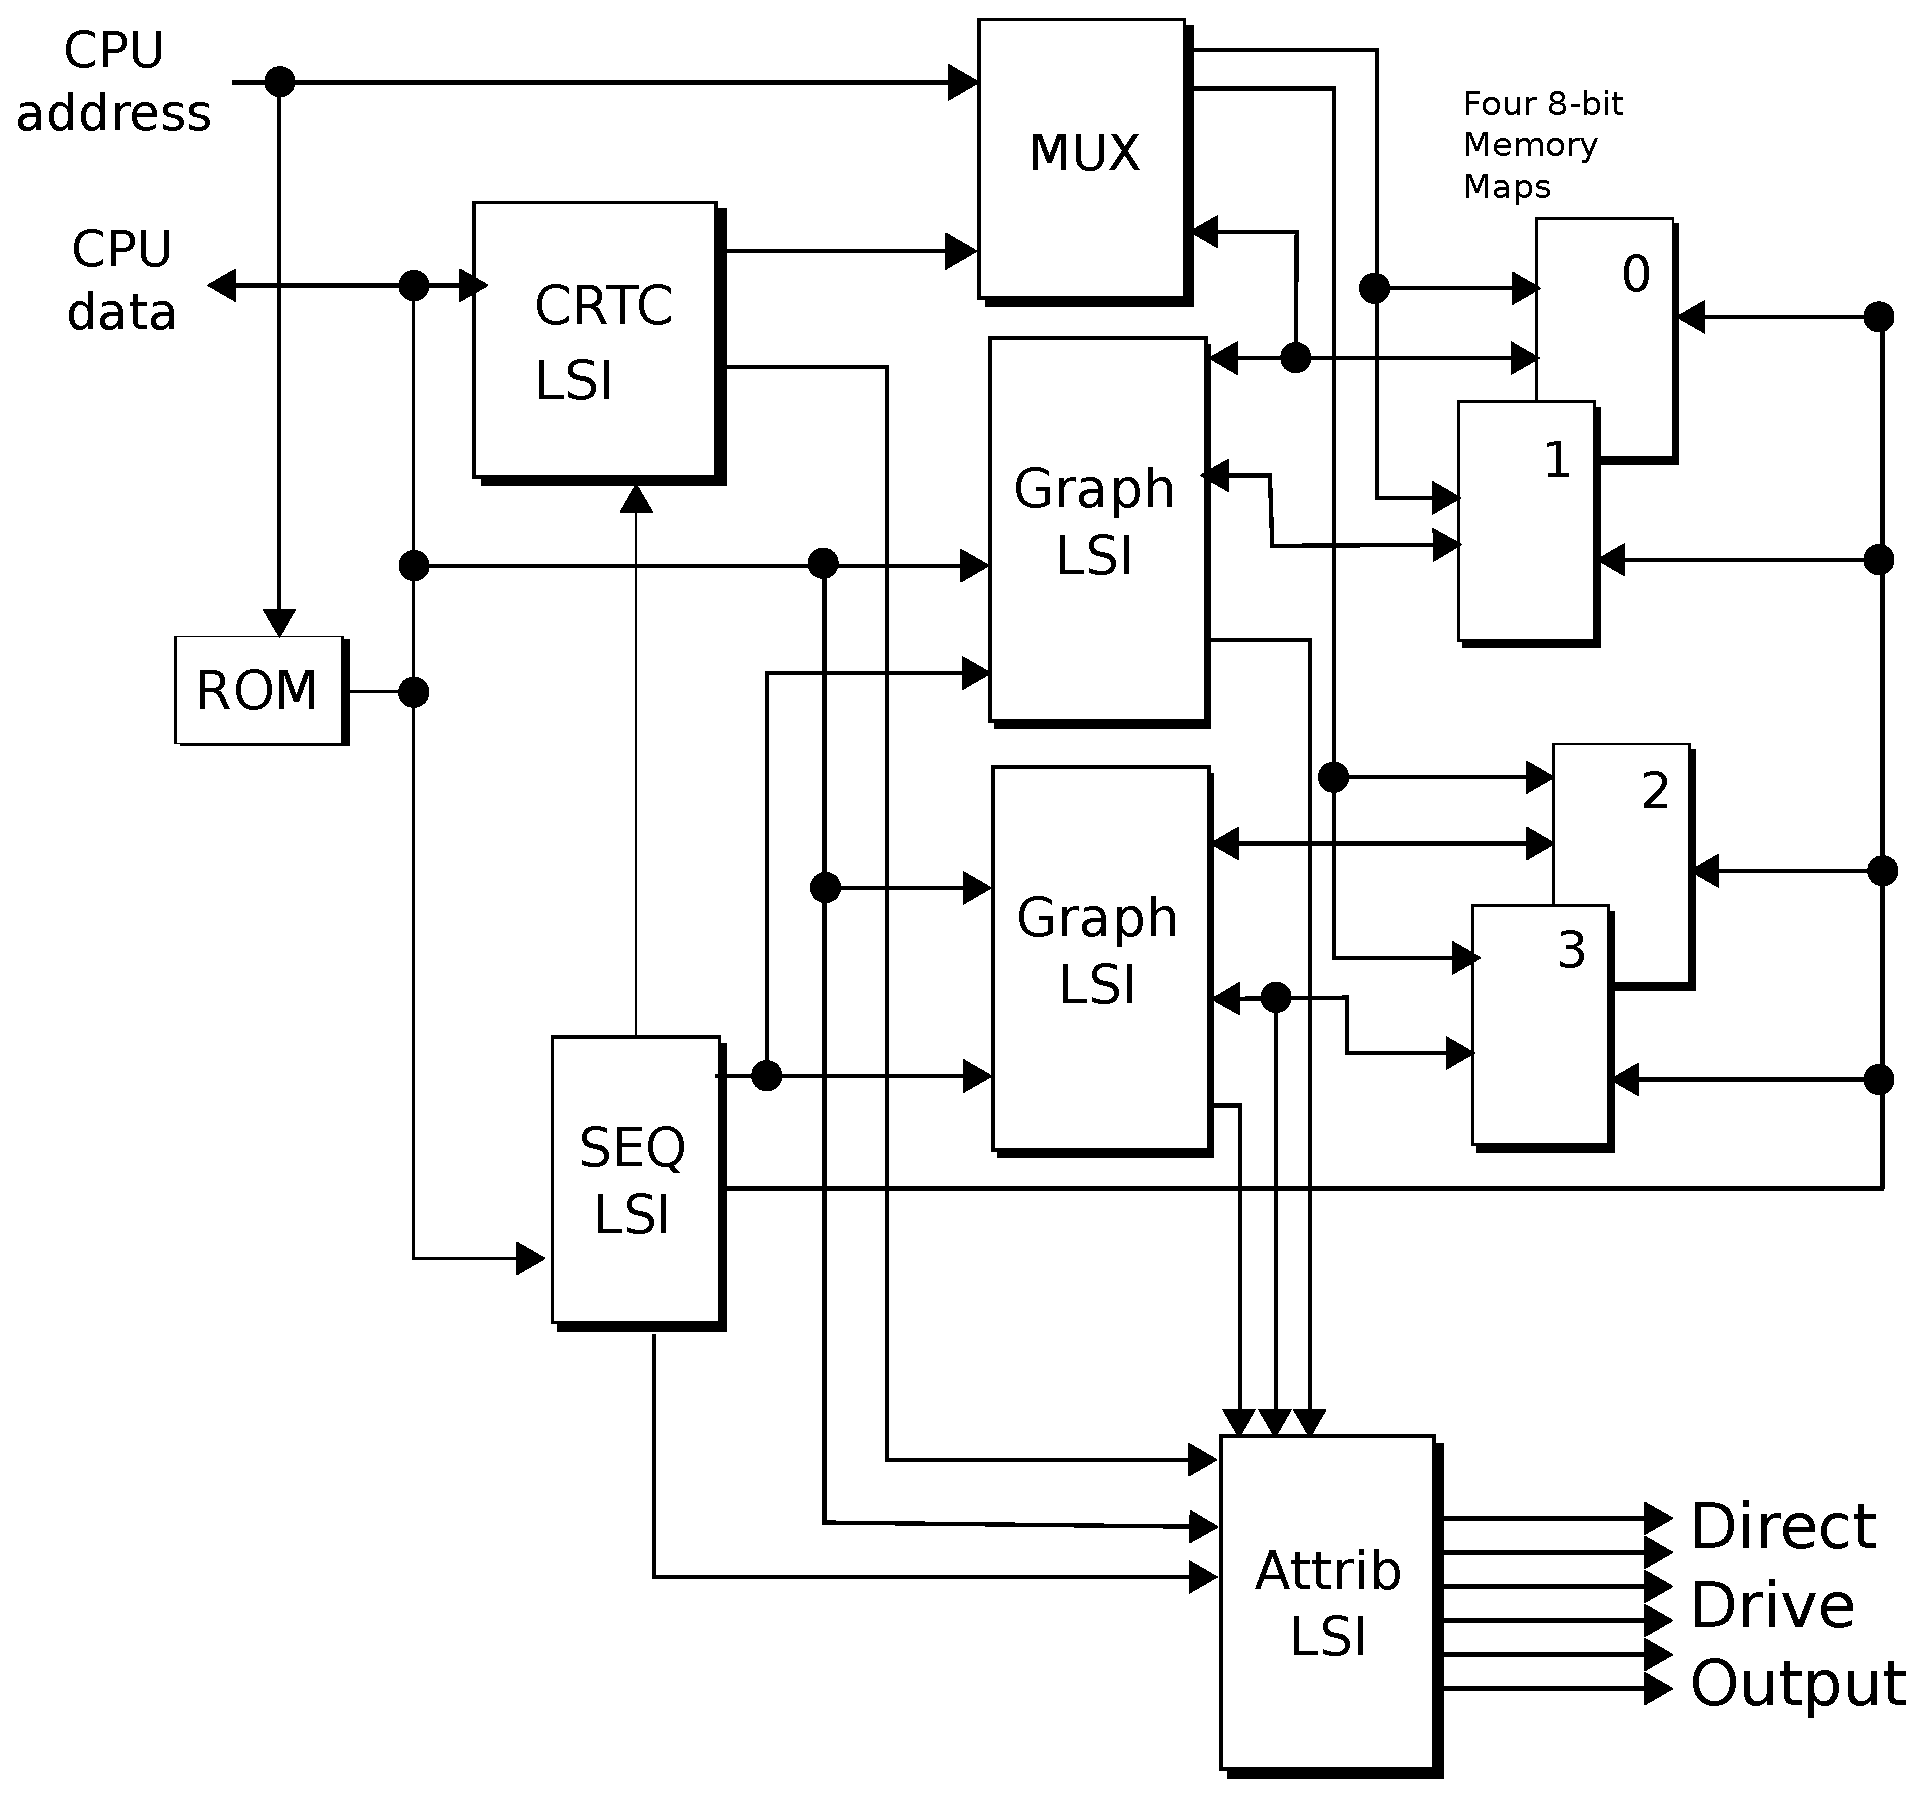
\includegraphics[width=0.9\textwidth]{imgs/drawings/ibm_ega.eps}
\caption{IBM's EGA documentation.}
\label{fig:ibm_ega}
\end{figure}

\par
The overall design can be simplified into several main components responsible for input, storage, and output:
\begin{itemize}
\item Two discrete Graphics Controllers to control and translate data between the CPU and video memory.
\item The framebuffer (VRAM), organized into four memory banks (planes), which stores the image data.  
\item The Sequencer Controller, which reads data from the four memory banks and converts it into color indices.
\item The CRT Controller and Attribute Controller, which convert color indices into synchronized RGBI signals and transmit them to the display using TTL\footnote{Transistor-Transistor Logic} signaling.
\end{itemize}

\par
\trivia{In the 1980's integrated video DACs\footnote{Digital to Analog Converter} were expensive and difficult to embed into custom chips. Most home computers with RGB output used TTL for digital output. With the introduction of VGA the DAC became the standard}.\\



\begin{figure}[H]
\centering
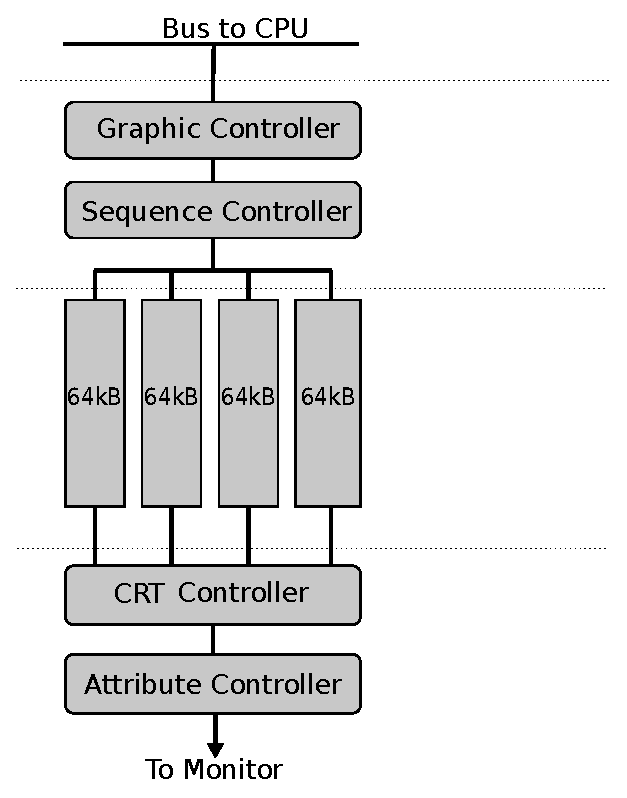
\includegraphics[width=0.8\textwidth]{imgs/drawings/ega.eps}
\caption{Simplified EGA architecture, it should not be considered 100\% correct.}
\label{fig:ega_arch}
\end{figure}

\par
A particularly interesting aspect of the architecture is the use of four memory banks. Let’s do some math to better understand why this architecture is chosen. A 640 x 350 image with 16 colors (4 bits per pixel) requires 640 x 350 x 4 bits = 896,000 bits, or 112KB of VRAM. This exceeds the 64KiB segment size imposed by the x86 Real Mode architecture, meaning the CPU could not access the entire framebuffer without performing relatively slow segment register changes while updating the screen.\\

\par
A second, more serious issue was memory bandwidth. To support a CRT refresh rate of 60 Hz, the adapter needed to provide one byte every $\frac{1}{112,000*60}=149$ nanoseconds. At the time, typical RAM access latency was around 200ns, which would have choked the video adapter.\\

\par
The EGA card solved these limitations by dividing memory into four planes and accessing them in parallel. This type of architecture is called "planar". This reduced the effective address space per plane by a factor of four, meaning each plane only needed to supply one byte every 596 nanoseconds, thereby relaxing the timing constraints on memory access.\\




\subsection{EGA Modes}
The EGA card remained backward compatibility with previous video adapters. In addition to introducing new, higher-resolution graphics modes, EGA retained support for both Monochrome Display Adapter (MDA) and Color Graphics Adapter (CGA) modes. This ensured that existing software written for earlier IBM PCs would continue to function without modification. \\ 


\vspace{-10pt}
\begin{figure}[H]
\centering
\begin{table}[H]
\begin{tabularx}{\textwidth}[c]{llllc}
\hline
\textbf{Mode} & \textbf{Type} & \textbf{Format} & \textbf{Colors} & \textbf{RAM Mapping}  \\ \hline
00h             & text          & 40x25           & 16 (monochrome) & B8000h    \\ \hline
01h             & text          & 40x25           & 16              & B8000h    \\ \hline
02h             & text          & 80x25           & 16 (monochrome) & B8000h    \\ \hline
03h             & text          & 80x25           & 16              & B8000h    \\ \hline
04h             & CGA Graphics  & 320x200         & 4               & B8000h    \\ \hline
05h             & CGA Graphics  & 320x200         & 4 (monochrome)  & B8000h    \\ \hline
06h             & CGA Graphics  & 640x200         & 2               & B8000h    \\ \hline
07h             & MDA text      & 9x14            & 4 (monochrome)  & B0000h    \\ \hline
0Dh           & EGA graphic   & 320x200         & 16              & A0000h    \\ \hline
0Eh           & EGA graphic   & 640x200         & 16              & A0000h    \\ \hline
0Fh           & EGA graphic   & 640x350         & 4               & A0000h    \\ \hline
10h           & EGA graphic   & 640x350         & 16 (out of 64)    & A0000h  \\ \hline
\end{tabularx}
\end{table}
\caption{EGA Modes available.}
\label{ega-modes-available}
 \end{figure}
 
\trivia{The Modes \cw{08h-0Ah}  are reserved for PCjr (or Tandy Graphics Adapter) graphics modes, which offered 160x200 with 16 colors, 320x200 with 16 colors and 640x200 with 4 colors. Modes \cw{0Bh} and \cw{0Ch} are reserved for internal EGA BIOS.}\\

\par
Changing the video mode is usually done using the \cw{0x10h} BIOS interrupt, which handles all kind of video display operations. Changes via the BIOS are regarded as a safe way to ensure all registers are setup properly.
  \par
  \lstinputlisting[ language={[x86masm]Assembler}]{code/ega_mode0d.c}
  

  
\subsection{EGA Memory Mapping}
\label{section:ega_memmap}
Accessing video memory on the PC was not as straightforward as it might seem. Instead of communicating with the video card through special I/O instructions, the system relied on memory mapping. The video card’s VRAM was mapped directly into the CPU’s address space---on the EGA beginning at \cw{A0000h}---so the processor could treat it like conventional system RAM. This allowed for faster and more flexible data transfers.\\

\par
However, this design introduced a new challenge: how do you fit 256KiB of video memory into a 64KiB segment? The solution was "bank switching", implemented through a mapping mask configured via the EGA registers. By configuring the mask first, a program can select which memory plane it wants to write to.

\begin{figure}[H]
  \centering
  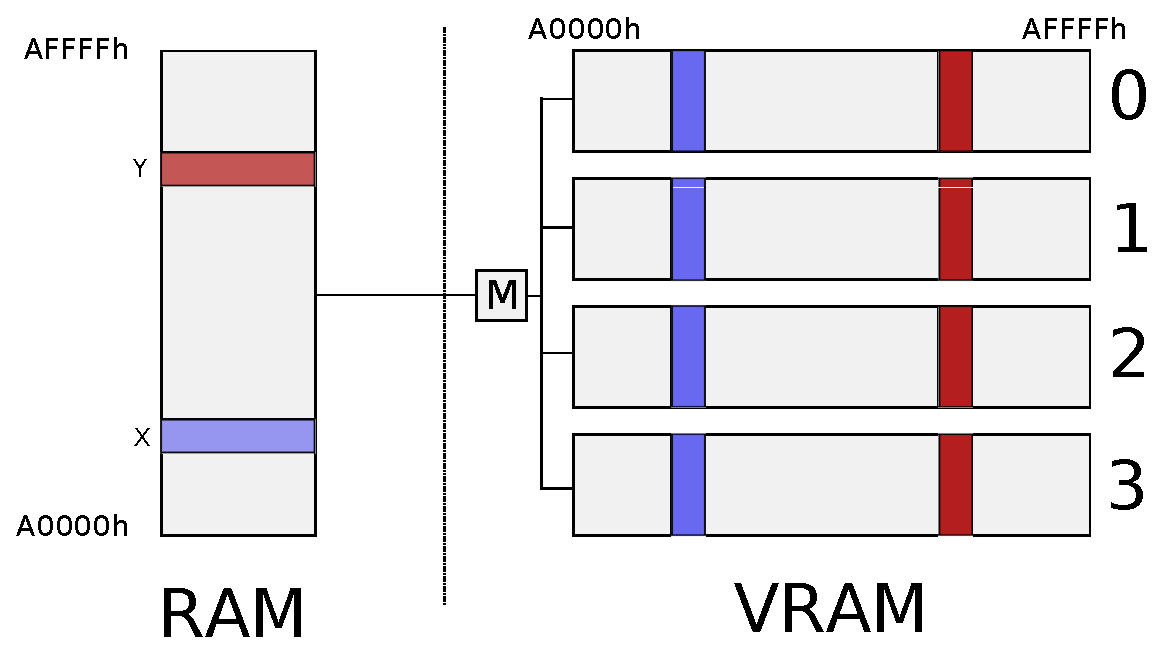
\includegraphics[width=1.0\textwidth]{imgs/drawings/ram_to_ega_mapping.eps}
  \caption{Mapping PC RAM to EGA VRAM banks.}
  \label{fig:ram_to_ega_mapping_label}
\end{figure}

\par
In mode \cw{0Dh}, each plane carries one bit of a pixel’s palette index. For EGA there are four planes, where combining one bit from each plane produces a 4-bit color index. This index is then translated into an on-screen color by the attribute controller, as illustrated below.\\

\par
To set the color of a single pixel, the programmer must write one bit in each of the four planes at the corresponding byte and bit position. Writing an individual pixel color was therefore CPU-intensive and should be minimized whenever possible.\\


\begin{figure}[H]
\centering
 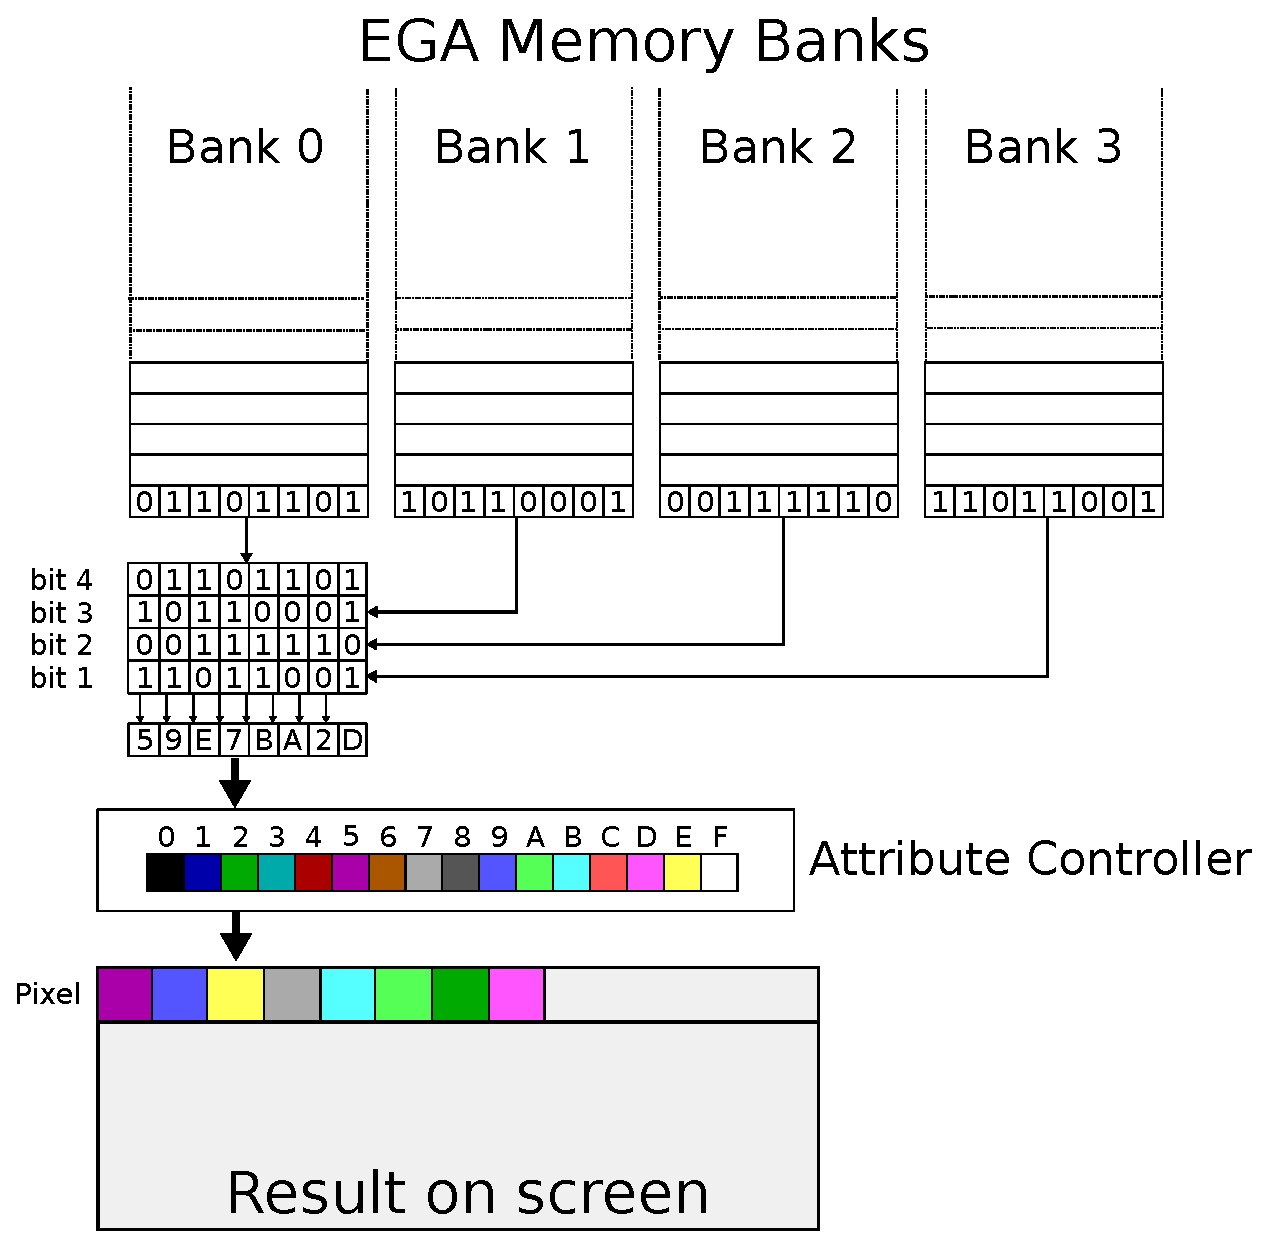
\includegraphics[width=1.0\textwidth]{imgs/drawings/mode0Dh.eps}
\caption{EGA mode 0Dh, how bank layout appears on screen.}
\label{fig:ega_bank_layout}
\end{figure}


\subsection{Programming on the EGA}	
In the days of the EGA, there were no graphics drivers to rely on and no Windows DirectX to smooth things over. Programming graphics truly meant programming on the bare metal via I/O port addresses. The EGA card had multiple I/O port addresses that are generally directed to one of the sub-components.

\vspace{8pt}
\begin{figure}[H]
\centering
\begin{tabularx}{\textwidth}[c]{|>{\hsize=.35\hsize}X |>{\hsize=.65\hsize}X |}
\hline
\textbf{Component}     & \textbf{I/O port address} \\ \hline
Miscellaneous          & \cw{3B2h}, \cw{3BAh}, \cw{3C2h}, \cw{3D2h}, \cw{2DAh} \\ \hline
CRT Controller         & \cw{3B4h}, \cw{3B5h}, \cw{3D4h}, \cw{3D5h} \\ \hline
Attribute Controller   & \cw{3C0h} 		\\ \hline
Sequence Controller    & \cw{3C4h}/\cw{3C5h}  \\ \hline
Graphics Controller    & \cw{3CCh}, \cw{3CAh}, \cw{3CEh}, \cw{3CFh} \\ \hline
\end{tabularx}
\caption{EGA I/O port addresses.}
\label{ega-IO-ports}
 \end{figure}


\par
In most cases, a component used one I/O address to select a parameter and another as a data register, allowing dozens of settings to be exposed and configured on the EGA card.
Mastering the EGA card, however, was far from straightforward. Its many registers, bit masks, and undocumented quirks demanded patience and deep hardware knowledge. Only few programmers truly learned how to control the card to its full potential.



 
  
\subsection{EGA Color Palette}
\label{sec:ega_color_palette}
The EGA CRTC does not expect RGB values to generate pixels. Instead, it is based on an index-based color palette system. Each pixel is a 4-bit index number, assigned to a color from the Attribute Controller. The default color palette is all 16 CGA colors, but it allows substitution of each of these colors with any one from a total of 64 colors.\\

When calculating the intended value in the 64-color EGA palette, the 6-bit number of the intended entry is of the form "rgbRGB" where a lowercase letter is the least significant bit of the channel intensity (\(\frac{1}{3}\) color intensity) and an uppercase letter is the most significant bit of intensity (\(\frac{2}{3}\) color intensity). The more intensity, the brighter the color is. For example, \cw{02h} will produce green, \cw{10h} will produce dim green and \cw{12h} will produce bright green. Each of the 16 color indexes could be reassigned to one color from the "rgbRGB" palette.
 

\begin{figure}[H]
\centering
\setlength{\tabcolsep}{2.8pt} % set border margin to 0
\begin{tabular}{|c|c|c|c|c|c|c|c|c|c|c|c|c|c|c|c|c|}
\hline 
 & 00h & 01h & 02h & 03h & 04h & 05h & 06h & 07h & 08h & 09h & 0Ah & 0Bh & 0Ch & 0Dh & 0Eh & 0Fh \\ \hline
 00h & \cellcolor{CGA_Black} & \cellcolor{CGA_Blue} & \cellcolor{CGA_Green} & \cellcolor{CGA_Cyan} & \cellcolor{CGA_Red} & \cellcolor{CGA_Magenta} & \cellcolor{EGA_06} & \cellcolor{CGA_Light_Grey} & \cellcolor{EGA_08} & \cellcolor{EGA_09} & \cellcolor{EGA_0A} & \cellcolor{EGA_0B} & \cellcolor{EGA_0C} & \cellcolor{EGA_0D} & \cellcolor{EGA_0E} & \cellcolor{EGA_0F} \\ \hline

10h & \cellcolor{EGA_10} & \cellcolor{EGA_11} & \cellcolor{EGA_12} & \cellcolor{EGA_13} & \cellcolor{CGA_Brown} & \cellcolor{EGA_15} & \cellcolor{EGA_16} & \cellcolor{EGA_17} & \cellcolor{EGA_18} & \cellcolor{EGA_19} & \cellcolor{EGA_1A} & \cellcolor{EGA_1B} & \cellcolor{EGA_1C} & \cellcolor{EGA_1D} & \cellcolor{EGA_1E} & \cellcolor{EGA_1F} \\ \hline

20h & \cellcolor{EGA_20} & \cellcolor{EGA_21} & \cellcolor{EGA_22} & \cellcolor{EGA_23} & \cellcolor{EGA_24} & \cellcolor{EGA_25} & \cellcolor{EGA_26} & \cellcolor{EGA_27} & \cellcolor{EGA_28} & \cellcolor{EGA_29} & \cellcolor{EGA_2A} & \cellcolor{EGA_2B} & \cellcolor{EGA_2C} & \cellcolor{EGA_2D} & \cellcolor{EGA_2E} & \cellcolor{EGA_2F} \\ \hline

30h & \cellcolor{EGA_30} & \cellcolor{EGA_31} & \cellcolor{EGA_32} & \cellcolor{EGA_33} & \cellcolor{EGA_34} & \cellcolor{EGA_35} & \cellcolor{EGA_36} & \cellcolor{EGA_37} & \cellcolor{CGA_Dark_Grey} & \cellcolor{CGA_Bright_Blue} & \cellcolor{CGA_Bright_Green} & \cellcolor{CGA_Bright_Cyan} & \cellcolor{CGA_Bright_Red} & \cellcolor{CGA_Bright_Magenta} & \cellcolor{CGA_Bright_Brown} & \cellcolor{CGA_White} \\ \hline


\end{tabular}\\
\setlength{\tabcolsep}{6pt} % reset border margin
\caption{EGA "rgbRGB" color palette (64 values from 00h to 3Fh)}
\end{figure}

\par
Both CGA and EGA cards use a female nine-pin D-subminiature (DE-9) connector for output to the monitor. However, the pin configurations for CGA and EGA are different. CGA’s color output follows the "RGBI" model, where "I" stands for Intensity, adding brightness to the RGB color. As a result, CGA can produce up to 16 colors. Compared to CGA, the EGA card redefines some pins of the DE-9 connector to carry the extended rgbRGB-color information. If the monitor were connected to a CGA card, these pins would not carry valid color information, and the screen might be garbled if the monitor were to interpret them as such.\\

\par
For example, if the color brown (rgbRGB = \cw{010100b}) is assigned to a color index, the resulting output on a CGA pin configuration appears as light red. This occurs because the secondary green pin ("r" in rgbRGB) is mapped to the Intensity pin in CGA mode, producing the color red with intensity rather than the expected brown.

\begin{figure}[H]
\renewcommand{\arraystretch}{0.9}
\centering
\begin{table}[H]
\begin{tabularx}{\textwidth}[c]{|>{\hsize=.16\hsize}X |>{\hsize=.42\hsize}X |>{\hsize=.42\hsize}X |}
\hline
\color{black} \textbf{Pin} & \color{black} \textbf{Mode 2: EGA mode (rgbRGB)} & \color{black} \textbf{Mode 1: CGA mode (RGBI)} \\
\hline
\color{black} 1 & \color{black} Ground &\color{black} Shield Ground \\
\hline
\color{black} 2 & \color{white}\cellcolor{EGA_I_Red} Secondary Red (Intensity) &\color{black}Signal Ground \\
\hline
\color{black} 3 & \color{white}\cellcolor{CGA_Red} Primary Red &\color{white}\cellcolor{CGA_Red} Red \\
\hline
\color{black} 4 & \color{black}\cellcolor{CGA_Green} Primary Green &\color{black}\cellcolor{CGA_Green} Green \\
\hline
\color{black} 5 & \color{white}\cellcolor{CGA_Blue} Primary Blue &\color{white}\cellcolor{CGA_Blue} Blue \\
\hline
\color{black} 6 & \color{black}\cellcolor{EGA_I_Green} Secondary Green (Intensity) &\color{white}\cellcolor{CGA_Dark_Grey}Intensity \\
\hline
\color{black} 7 & \color{white}\cellcolor{EGA_I_Blue} Secondary Blue (Intensity) &\color{black}Reserved \\
\hline
\color{black} 8 & \color{black} Horizontal Sync &\color{black}Horizontal Sync \\
\hline
\color{black} 9 & \color{black} Vertical Sync &\color{black}Vertical Sync \\

\hline

\end{tabularx}
\end{table}
\caption{EGA and CGA DE-9 connector pin signals.}
\label{pin_signals}
 \end{figure}

\par
So how did an EGA monitor recognize that it was connected to an EGA video card? in fact, it could only distinguish EGA and CGA cards based on the Vertical Sync signal (pin 9), which is either 200- or 350-line mode. If the Vertical Sync is 350-line mode, the monitor switched to Mode 2 operation which supported the extended rgbRGB-color information\footnote{IBM Enhanced Color Display technical documentation}. But in the 200-line mode, the monitor cannot distinguish between being connected to a CGA or an EGA card. \\

\par
For this reason, EGA monitors use the CGA pin assignment for all 200-line modes (mode 1), allowing them to accept the same RGBI signal format as a CGA card. This makes an EGA monitor compatible with CGA output in those modes. Thereby it is able to show all 16 CGA colors simultaneously, whereas a CGA card is limited to four colors at once in graphics modes. The downside is that the 64-color EGA palette can only be used in 350-line mode.

\begin{figure}[H]
\renewcommand{\arraystretch}{0.9}
\centering
\begin{table}[H]
\begin{tabularx}{\textwidth}[c]{+X +X +X +X }
\hline
\textbf{\color{black}Index Number} & \textbf{\color{black}Color} & \textbf{\color{black}rgbRGB} & \textbf{\color{black}RGBI} 	\\ \hline
\rowcolor{CGA_Black}\rowstyle{\color{white}} 00h & Black          & 000000b           & 0000b 	\\ \hline
\rowcolor{CGA_Blue} 01h & Blue          & 000001b           &  0010b  			\\ \hline
\rowcolor{CGA_Green} 02h & Green          & 000010b           & 0100b   			\\ \hline
\rowcolor{CGA_Cyan} 03h & Cyan          & 000011b           & 0110b   			\\ \hline
\rowcolor{CGA_Red} 04h & Red          & 000100b           & 1000b   				\\  \hline
\rowcolor{CGA_Magenta} 05h & Magenta          & 000101b           & 1010b   		\\ \hline
\rowcolor{CGA_Brown} 06h & Brown          & 010100b           & 1100b   		\\ \hline
\rowcolor{CGA_Light_Grey} 07h & Light grey          & 000111b           & 1110b	\\ \hline
\rowcolor{CGA_Dark_Grey} 08h & Dark grey          & 111000b           & 0001b   		\\ \hline
\rowcolor{CGA_Bright_Blue}\rowstyle{\color{black}} 09h & Bright blue          & 111001b           & 0011b   			\\ \hline
\rowcolor{CGA_Bright_Green} 0Ah & Bright green          & 111010b   & 0101b	\\ \hline
\rowcolor{CGA_Bright_Cyan} 0Bh & Bright cyan          & 111011b     & 0111b   			\\ \hline
\rowcolor{CGA_Bright_Red} 0Ch & Bright red          & 111100b           & 1001b			\\ \hline
\rowcolor{CGA_Bright_Magenta} 0Dh & Bright magenta          & 111101b           & 1011b   		\\ \hline
\rowcolor{CGA_Bright_Brown} 0Eh & Yellow          & 111110b           & 1101b	\\ \hline
\rowcolor{CGA_White} 0Fh & White          & 111111b           & 1111b   		\\ \hline
\end{tabularx}
\end{table}
\caption{Default EGA 16-color palette}
\label{default_ega_palette}
 \end{figure}

\trivia{The color brown (\cw{06h}) is actually dark yellow. IBM engineers found this shade unappealing, so they implemented a special hack in the monitor that targets color \cw{06h}. When detected, the monitor halves the green intensity, producing a golden brown instead of dark yellow.}\\


\section{Audio}
\label{hardware-audio}
For the first 5-6 years of the IBM PC and its compatibles, their audio output came from nothing more than a simple loudspeaker with a tone generator. For business, this was acceptable - even preferable, since a PC in an office environment really shouldn't be a distraction to others! The loudspeaker, commonly known as a "PC Speaker", was capable of generating a square wave via 2 levels of output.\\
\begin{figure}[H]
\centering
\scaledimage{0.6}{pcspeaker.png}
\end{figure}


\subsection{History of Sound Cards}
The introduction of real game music and sounds on the PC started with Sierra back in 1988. They prepared to change all this by creating games that contained serious, high quality musical compositions drawing on add-on hardware. \textit{King's Quest IV} was the first commercially released game for IBM PC compatibles to support sound cards. In addition to the familiar PC speaker and Tandy 1000, it could utilize 
\begin{itemize}
    \item Roland MT-32
    \item IBM Music Feature Card
    \item AdLib
\end{itemize}
 
Sierra struck a deal with two companies, Roland and AdLib, where Sierra would also become a reseller for these soundcards. \\

\par
The Roland MT-32 was the higher end of these music devices. In today's terminology, it would be labeled a "Wavetable Synthesizer". A wavetable synthesizer usually implies that real instrument sounds are recorded into the hardware of the device. This device can then manipulate them to play them back at the various notes you need. The MT-32 had the ability to manipulate parts of its built-in sounds using something called "Linear Arithmetic (LA)" synthesis. It was a very good device that can rival even today's sound cards. To connect the MT-32 to a PC required, what Roland called an MPU-401\footnote{Midi Processing Unit-401}, in one of the PC's expansion slots. Sierra sold the MT-32 with a necessary MPU-401 interface for \$550. The high price prevented it from dominating the end-user market of gaming.\\

\par
  \begin{figure}[H] 
    \centering 
    \scaledimage{.7}{hardware/MT_32.png} 
    \caption{Roland MT-32 synthesizer box.}
  \end{figure}


\par
The IBM Music Feature Card was launched in March 1987 as a collaboration between IBM and Yamaha. Essentially the Music Feature Card was a synthesizer installed on an 8-bit expansion card\footnote{Roland released the LAPC-I in 1989, which basically was similar to the Music Feature Card: a MT-32-compatible Roland synthesizer with a MPU-401 unit, integrated onto one single full-length 8-bit ISA card.}. The Music Feature Card had 8 FM voices, controlled via 4 frequency operators. It came with over 300 high-quality synthesized instruments on-board, and it was actually possible to have two Music Feature Cards in a single PC to get 16 voices. With a tag price of \$495 it was just like the Roland MT-32 an expensive card, and its audience was primarily business users.\\

\par
  \begin{figure}[H] 
    \centering 
    \scaledimage{1.0}{hardware/IBM_Music_Feature.png} 
    \caption{IBM Music Feature Card.}
  \end{figure}




 \subsection{AdLib}
AdLib was the other company, beside Roland, that struck a deal with Sierra as a reseller. The company was founded in 1987 by Martin Prevel, a former professor of music from Quebec. The AdLib soundcard used a technology called FM synthesis. The technology is based on the idea of generating superimposing waveforms to create a sound. This technology was much less expensive than Roland's Wavetable technology.\\

\par
The AdLib card was built around the Yamaha YM3812, also known as the OPL2 chip, and could produce either 9 sound channels or 6 sound channels plus 5 hit instruments simultaneously using Frequency Modulation (FM). Ideally, if you have enough generators and can fine tune the waveforms well enough, you can create a realistic sound. However, to reach this ideal, you need lots of skilled people, lots of money for equipment, and lots of time to develop. Thus, FM synthesis sounded very artificial. Still, this was a great improvement over the PC Speaker. With a price tag of \$219.99, it was much cheaper than the Roland MT-32 and IBM Music Feature Card, and soon ruled at the top of the early PC sound card market.\\

\par
  \begin{figure}[H] 
    \centering 
    \scaledimage{.85}{hardware/adlib_1.5.png} 
    \caption{An AdLib sound card. Notice the big YM3812 chip.}
  \end{figure}

\par
The AdLib card dominated the PC market for almost three years. Then, in 1989, Creative Labs released the competing SoundBlaster, which quickly dominated over AdLib. To compete with SoundBlaster, AdLib planned a new 12-bit stereo sound card called AdLib Gold. Sadly, due to AdLib's dependence on Yamaha who suffered long delays introducing their latest multimedia chipset, their new product, AdLib Gold PC-1000, was never to see the light of day under AdLib's management. Unable to remain solvent, AdLib closed its doors on 1\textsuperscript{st} May 1992.\\





  \subsection{SoundBlaster}
  Creative Labs, the company behind the SoundBlaster, didn't enter the sound card industry until 1987 with the introduction of their Creative Music System (C/MS). From inception in 1981, they were a computer repair shop in Singapore. Creative Music System, or "Game Blaster" as it was renamed a year later, was a FM synthesizer card similar to AdLib. Based on the Philips SAA1099 chip, which was essentially a square-wave generator, it sounded much like twelve simultaneous PC speakers would have, except for each channel having amplitude control. The card did not sell well.\\
  
  \par
The original Sound Blaster v1.0 and v1.5 were released in 1989 as the successor to the Game Blaster. Not only was it equipped with the OPL2 chip, providing 100\% compatibility with AdLib music playback, but it was also technologically superior with a DSP\footnote{An Intel MCS-51 "Digital Sound Processor", not "Digital Signal Processor".} allowing PCM playback (digitized sounds) at 8 bits per sample and up to 22.05 kHz sampling rate. The card also came with a DA-15 port allowing joystick connection. Most importantly, the Sound Blaster was \$90 cheaper than the AdLib, which led many consumers to choose it instead. In less than a year, the Sound Blaster became the top-selling expansion card for the PC. \\

\par
\begin{fancyquotes}
At Comdex [1989], we sold one Sound Blaster every four minutes.\\ 
\par
\textbf{Sim Wong Hoo, founder, on their rapid success}
\end{fancyquotes}\\

\par
Figure \ref{asb15} is the SoundBlaster model CT1320B. Notice the OPL2 chip (labeled FM1312) and the CT1321 DSP on the middle top. In the middle of the card are the two CMS-301 chips, to ensure backwards compatibility with the Creative Music System. The CT1320B model (Sound Blaster 1.5) was a cost-cutting measure. Having recognized that C/MS was unpopular, they replaced the two C/MS chips with sockets. You could still purchase the C/MS chips for \$29.95 if you wished and install them into these sockets.\\
  
\begin{figure}[H] 
  \centering 
  \scaledimage{1.0}{hardware/Soundblaster-ct1320.png} 
\end{figure}

\begin{figure}[H] 
  \centering 
  \includegraphics[width=1.0\textwidth]{imgs/drawings/soundblaster_layout.eps}
  \caption{A SoundBlaster 1.5, model CT1320B }
  \label{asb15}
\end{figure}  

  
\par
  \trivia{Creative Labs boasts in their own advert AdLib compatibility and even uses an image of AdLib Inc's product\footnote{Advert p20 in Compute!, April 1990.}! On the other hand, they sued every company that tried to market a 'Sound Blaster compatible' product for using the name of their product.}\\

\begin{figure}[H] 
  \centering 
  \scaledimage{0.98}{hardware/sound_blaster_box_front.jpg} 
  \caption{Sound Blaster advertisement with Adlib compatibility.}
  \label{asb15_advertise}
\end{figure}


  
  

\section{Floppy Disk Drive}
Before the internet, floppy disks were the primary medium for sharing and distributing software and data. The original XT systems were equipped with 5\nicefrac{1}{4}-inch floppy disk with a capacity of 360KiB\footnote{Manufactureres often rounded this down to 360K or 360KB for simplicity, using the decimal definition of KB (1000 bytes) in marketing.}. In 1984, IBM introduced with its PC AT the 1.2MB dual-sided 5\nicefrac{1}{4}-inch floppy disk, but it never became very popular. IBM started using the 720KiB double density 3\nicefrac{1}{2}-inch floppy disk in 1986 and the 1.44MB high-density version in 1987. The advantages of the 3\nicefrac{1}{2}-inch disk were its higher capacity, its smaller physical size, and its rigid case which provided better protection from dirt and other environmental risks. By the mid-1990s, 5\nicefrac{1}{4}-inch drives had virtually disappeared, as the 3\nicefrac{1}{2}-inch disk became the predominant floppy disk. \\

\vspace{10pt}
\trivia{An USB stick of 128GB contains more than 91K high-density 3\nicefrac{1}{2}-inch (1.44MB) floppy disks.}\\
\par

\begin{figure}[H]

  \begin{minipage}{0.48\textwidth}
  \centering
  \scaledrawimage{4cm}{hardware/floppy_3_1_2.png} 
  \end{minipage}
  \hfill
  \begin{minipage}{0.48\textwidth}
  \centering
  \scaledrawimage{6cm}{hardware/floppy_5_1_4.png}
  \end{minipage}
  \caption{3\nicefrac{1}{2}-inch and 5\nicefrac{1}{4}-inch floppy disk.}
  \end{figure}
\par


A floppy disk is essentially a very flexible piece (hence the term floppy disk) of plastic coated on both sides in a magnetic material. This "disk" of plastic is contained within a protective envelope or hard plastic case, which is then inserted into the drive and automatically locked onto a spindle. It is then rotated at a constant speed, 360 rpm for standard PC floppy drives. A head assembly consisting of two magnetic read/write heads, one in contact with the upper surface and one in contact with the lower surface of the disk, may be moved in discrete steps across the disk and read the data from the disk.\\

\par
The data on a floppy disk is stored in concentric circular tracks divided into arc-shaped sectors. The amount of data a disk can store is determined by the number of tracks and sectors and the density of the recorded information (single and double density). Near the center, there is a small hole called the index hole, which marks the start of a sector.\\

\begin{figure}[H]
\centering
      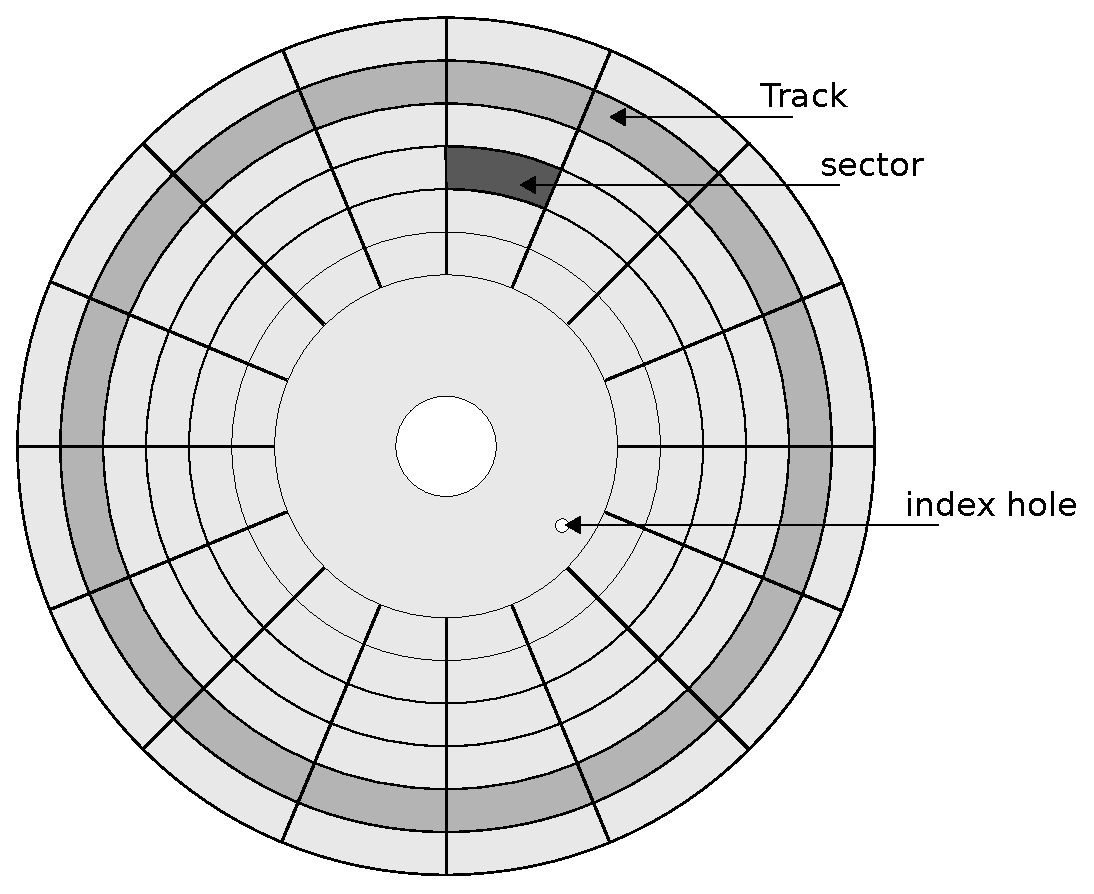
\includegraphics[width=0.7\textwidth]{imgs/drawings/floppy_disk.eps}
      \caption{Floppy disk with tracks, sectors and the index hole.}
\end{figure} 

\par
When the floppy disk drive is powered up, the read/write heads move to the target track, starting from track 0 (the starting track on a floppy disk). Once the sensor reaches the target track, the computer is ready to retrieve or write data onto the floppy disk. To select a specific sector, the drive must wait for that sector to pass under the head. The drive determines which sector it is on by waiting for the index hole to be under the head. Since the rotation speed is kept constant, the time when the next sector is under the head is known. Now, the head can read or write to the specific sector/track combination on the disk.\\


\par
The floppy disk is controlled via the Floppy Disk Controller (FDC), and a typical read operation from the floppy disk contains the following steps:
\begin{itemize}
  \item Turn the disk motor on. When you turn a floppy drive motor on, it takes quite a few milliseconds to "spin up", to reach the (stabilized) speed needed for data transfer.
  \item Perform seek operation, which moves the head to the correct location for reading the data.
  \item Read the data from the floppy disk and store the data via the FDC to RAM memory.
  \item Turn the disk motor off. 
\end{itemize}

The controller waited a few seconds before turning off the motor. The reason to leave the motor on for a few seconds is that the controller may not know if there is a queue for sector reads or writes that are going to be executed next. If there are going to be more drive accesses immediately, they won't need to wait for the motor to spin up again.\\

\section{Keyboard}
The original IBM PC and XT keyboards featured 83 keys. After receiving feedback from users frustrated by the layout, IBM introduced the 84-key PC AT keyboard, which included a rearranged layout and the addition of the "Sys Req" key. It also introduced 3 status LEDs for Caps Lock, Num Lock and Scroll Lock.

\begin{figure}[H] 
  \centering 
  \scaledimage{0.95}{hardware/keyboard_AT.png} 
  \caption{IBM AT Keyboard.}
\end{figure}

\par
This design was further updated in 1986 with the release of the IBM Model M. It officially became the IBM PC standard in 1987 with the introduction of the IBM Personal System/2 (PS/2). The function keys were moved to the top, F11 and F12 were added, and the total number of keys increased to 101 (ANSI) or 102 (ISO). The Model M was widely adopted and is still being used today.\\

\par
The IBM Model M came in two main versions: the ANSI layout with 101 keys for the US and Canada, and the ISO layout with 102 keys, primarily used in Europe and other international markets. The primary differences between both layouts are the shape of the Enter key, the size of the left Shift key, and the presence of an extra key on the ISO variant to provide better support for typing in multiple languages with accents and special characters.

\begin{figure}[H] 
  \centering 
  \scaledimage{0.95}{hardware/keyboard_PS2.png} 
  \caption{IBM Keyboard model M 101-key layout (PS/2).}
\end{figure}

At the time, keyboards were connected either via PS/2 or AT ports.\\

\par
\begin{figure}[H]
  \centering
  \begin{subfigure}{.5\textwidth}
    \centering
    \includegraphics[width=0.25\textwidth]{imgs/drawings/ports/MiniDIN-6_PS2.eps}
  \end{subfigure}%
  \begin{subfigure}{.5\textwidth}
    \centering
    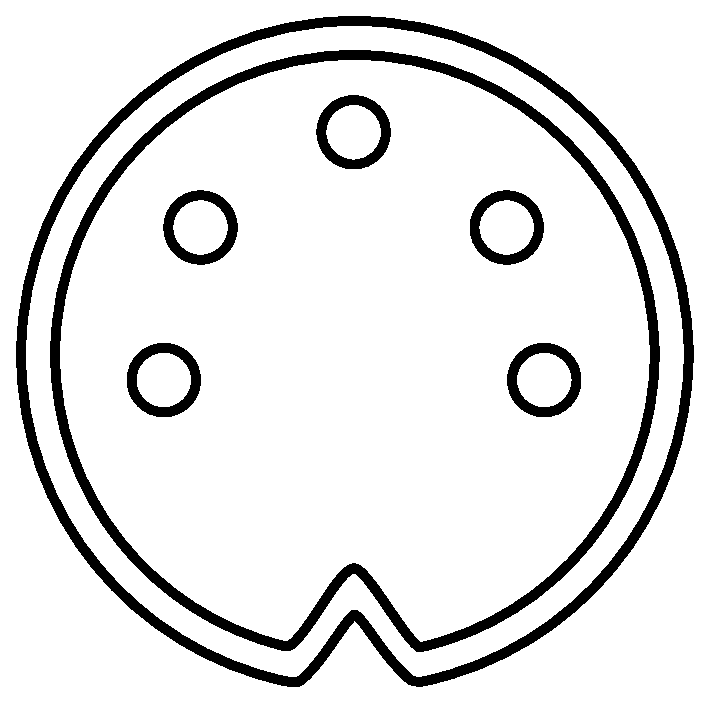
\includegraphics[width=0.25\textwidth]{imgs/drawings/ports/AT_Diagram.eps}
  \end{subfigure}
  \caption{PS/2 (left) and AT (right) keyboard connector.}
  \label{fig:keyboard_connector}
\end{figure}


\section{Summary}
To say a PC was difficult to program for games would be an understatement. It was a nightmare. The CPU was good at doing the wrong thing, the best graphic interface had a complex architecture to write a single pixel to the screen, different keyboard layouts, and a memory model only allowed 1 MiB with an address composed of two separate 16-bit registers. Last, but not least, the default sound system could only produce square waves and sound cards were in a very early stage of development.\\

\par
Yet despite all these unfavorable conditions, teams of developers gathered to tame the beast and unleash its power to gamers. One of these called themselves \textit{Ideas From the Deep}\footnote{Throughout the book, \textit{Ideas from the Deep} and \textit{id Software} will be used interchangeably.}.
\end{document}




